%% Template.tex; Solar Physics
%% 
\documentclass[namedreferences]{SolarPhysics}
%
% spr-sola-addons available options:
%  natbib        -- For citations: redefine \cite commands
%  solaenum      -- makes enumerated list with italics-roman numerals and a single right-bracket
%  linksfromyear -- loads a natbib and puts a link on a year citation (hyperref must be loaded)
%  optionalrh    -- for optional running title/author
%
%\usepackage[optionalrh,solaenum]{spr-sola-addons} % For Solar Physics 
%\usepackage{epsfig}                     % For eps figures, old commands
\usepackage{graphicx}                    % For eps figures, newer & more powerfull
%\usepackage{courier}                    % Change the \texttt command to courier style
%\usepackage{amssymb}                    % useful mathematical symbols
\usepackage{color}                       % For color text: \color command
\usepackage{url}                         % For breaking URLs easily trough lines
\def\UrlFont{\sf}                        % define the fonts for the URLs

%% Local definitions
%% please place your own definitions here and don't use \def but
%% \newcommand{}{} or 
%% \renewcommand{}{} if it is already defined in LaTeX

%I'm adding these:
\usepackage[optionalrh,natbib]{spr-sola-addons}
\newcommand{\solphys}{{\it Solar Physics}}
\newcommand{\aap}{    {\it Astronomy \& Astrophysics}}
\newcommand{\aaps}{   {\it Astronomy \& Astrophysics Supplemental}}
\newcommand{\apj}{    {\it Astrophysical Journal}}



%%%%%%%%%%%%%%%%%%%%%%%%%%%%%%%%%%%%%%%%%%%%%%%%%%%%%%%%%%%%%%%%%%
\begin{document}

\begin{article}

\begin{opening}

\title{A Multiscale Technique for Automatically Detecting and Tracking CMEs in Coronagraph Data}

%%%%%%%%%%%%%%%%%%%%%%%%%%%%%%%%%%%%%%%%%%%%%%%%%%%
%% Authors Names
%
\author{J.~P.~\surname{Byrne}$^{1}$\sep
        H.~\surname{Morgan}$^{1}$\sep
        S.~R.~\surname{Habbal}$^{1}$      
       }

%%%%%%%%%%%%%%%%%%%%%%%%%%%%%%%%%%%%%%%%%%%%%%%%%%%
%% Runningheads
%
\runningauthor{J.~P.~Byrne {\it et al.}}
\runningtitle{Multiscale Technique for Automatically Detecting and Tracking CMEs}


%%%%%%%%%%%%%%%%%%%%%%%%%%%%%%%%%%%%%%%%%%%%%%%%%%%
%% Affilations 
%
  \institute{$^{1}$ Institute for Astronomy, University of Hawaii, 2680 Woodlawn Drive, Honolulu, HI 96822, USA
                     email: \url{jbyrne@ifa.hawaii.edu} email: \url{hmorgan@ifa.hawaii.edu} email: \url{shadia@ifa.hawaii.edu}%\\ 
%             $^{2}$ Second affiliation
%                     email: \url{e.mail-c} \\
             }


%%%%%%%%%%%%%%%%%%%%%%%%%%%%%%%%%%%%%%%%%%%%%%%%%%%
%%% Abstract 
\begin{abstract}
Studying coronal mass ejections (CMEs) in coronagraph data can be challenging due to their diffuse structure and transient nature, and user-specific biases may be introduced through visual inspection of the images. The large amounts of data available from the SOHO, STEREO, and future Solar Orbiter missions, also makes manual cataloguing of CMEs tedious, and so a robust method of detection and analysis is required. This has led to the development of automated CME detection and cataloguing packages such as CACTus, SEEDS and ARTEMIS. However, the main drawbacks of these catalogues are: the CACTus method of detection fails to resolve CME acceleration profiles; the CACTus and SEEDS running-difference images suffer from spatiotemporal crosstalk; and the SEEDS and ARTEMIS detections are limited to only the LASCO/C2 field-of-view. Recently, the benefits of multiscale filtering of coronagraph data have been demonstrated in an effort to overcome current cataloguing issues. A multiscale decomposition can be applied to individual images in order to enhance the structure of CMEs whilst removing noise and small-scale features like stars. Here we present the development of a new, automated, multiscale, CME detection \& tracking technique. It works by first separating the dynamic CME signal from the background corona and then characterising CME structure via a multiscale edge-detection algorithm. The detections are then chained through time to determine the CME kinematics and morphological changes as it propagates across the plane-of-sky. We demonstrate its application to a sample of LASCO data and prove its efficacy in detecting and tracking CMEs. This technique is being applied to the complete LASCO dataset, and it is planned to further develop it for implementation on the SECCHI/COR dataset in the near future.
\end{abstract}



%%%%%%%%%%%%%%%%%%%%%%%%%%%%%%%%%%%%%%%%%%%%%%%%%%%
%% Keywords
%
%\keywords{}


\end{opening}
%-------------------------------------------------

%%%%%%%%%%%%%%%%%%%%%%%%%%%%%%%%%%%%%%%%%%%%%%%%%%%
%% Sections
%
% \section{}%\label{s:?} 

\section{Detecting and Tracking CMEs}


In coronagraph images CMEs are observed as outwardly moving regions of stronger brightness intensities relative to the background corona. Different approaches to thresholding the intensity of CMEs in these images have been employed in order to detect their appearance and track their motion through the field-of-view, leading to a cataloguing of their kinematics and morphology. However, these techniques suffer several drawbacks and, as such, different catalogues can vary significantly in their description of events. We introduce a method of multiscale analysis to overcome certain drawbacks of previous detection and tracking methods. In multiscale decompositions of images, noise and small-scale features are removed to leave only larger-scale features of interest such as CMEs. This allows them to be tracked through the image sequences in order to determine their changing kinematics and morphology. Unfortunately coronal streamers tend to appear on similar size scales to CMEs, making their automatic detection difficult. Streamers do, however, tend to remain static on timescales comparable to CME propagation through the field-of-view, and contain much less angular information than the typically curved structure of CMEs, so they may be removed through spatio-temporal filtering of multiscale CME images. This chapter discusses the previous CME detection catalogues, and outlines our use of new methods of multiscale filtering to detect the CME edges in single images. We discuss our efforts to extend this to an automated CME detection algorithm. We also outline an ellipse characterisation of the CME front for study.

\subsection{CME Detection Catalogues}
\label{sect:cmecatalogues}

Current methods of CME detection have their limitations, mostly since these diffuse objects have been difficult to identify using traditional image processing techniques. These difficulties arise from the varying nature of the CME morphology, the scattering effects and non-linear intensity profile of the surrounding corona, the presence of coronal streamers, and the addition of noise due to cosmic rays and solar energetic particles (SEPs) that impact the coronagraph detectors. The images are also prone to numerous instrumental effects and possible data dropouts.  The following standard preprocessing methods are usually applied to optimise the images for CME studies. The coronagraph images are normalised with regard to exposure time in order to correct for temporal variations in the image statistics. A filter may be applied to remove pixel noise, for example to replace hot pixels with a median value of the surrounding pixel intensities, or to reduce the effects of background stars in the image. A correction for vignetting effects and/or lens distortion may be applied to the images. A background subtraction may also be applied, obtained from the minimum of the daily median pixels across a time span of a month. The occulting disc is normally masked, along with any data drop-outs in the images. These steps lead to a clear improvement in the image quality for CME study (Figure~\ref{init_rm}).

\begin{figure}[!t]
\centerline{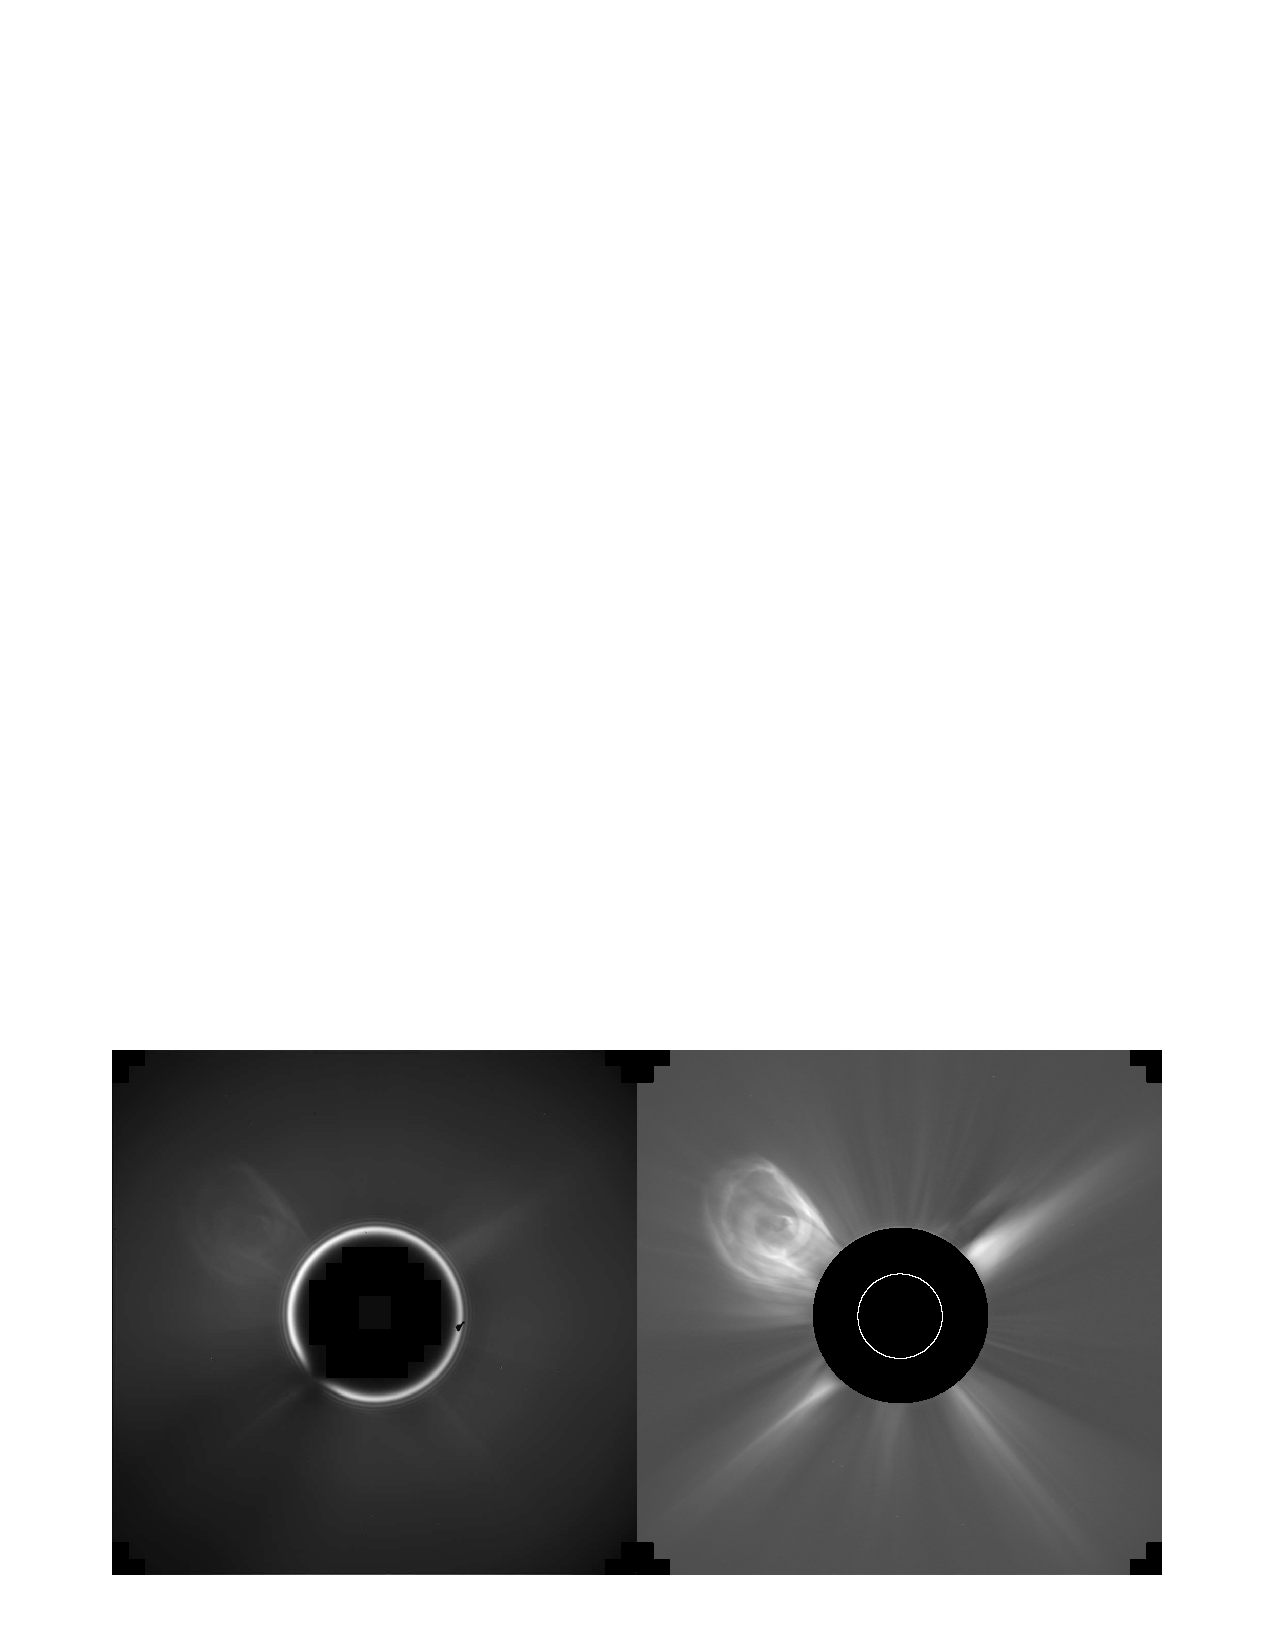
\includegraphics[scale=0.8, clip=true, trim=0 30 0 500]{images/normalising.pdf}}
\caption{Raw (left) and pre-processed image (right) of a CME observed by LASCO/C2 on 1 April 2004. The pre-processing includes normalising the image statistics, subtracting the background, and masking the occulter disk. The white circle (right) indicates the relative size and position of the Sun behind the occulter.}
\label{init_rm}
\end{figure}

\subsubsection{CDAW}

The CME catalogue hosted at the Coordinated Data Analysis Workshop (CDAW\footnote{http://cdaw.gsfc.nasa.gov/CME\_list}) Data Center grew out of a necessity to record a simple but effective description and analysis of each event observed by SOHO/LASCO \citep{2009EM&P..104..295G}. The catalogue is wholly manual in its operation, with a user tracking the CME through C2 and C3 running-difference images and producing a height-time plot of each event. A linear fit to the height-time profiles provides a 1st-order estimate for the plane-of-sky velocity, and a quadratic fit then provides a 2nd-order velocity fit and an acceleration for the event. The central position angle and angular width of the CME are also deduced from the images, and the event flagged as a halo if it spans 360$^{\circ}$, partial halo if it spans $\ge$\,120$^{\circ}$, and wide if it spans $\ge$\,60$^{\circ}$. The catalogue itself lists each CME's first appearance in C2, central position angle, angular width, linear speed, 2nd-order speed at final height, 2nd-order speed at 20~R$_{\odot}$, acceleration, mass, kinetic energy, and measurement position angle (the angle along which the heights of the CME are determined). While the human eye is supremely effective at distinguishing CMEs in coronagraph images, errors may be introduced to the manual cataloguing procedure through the biases of different operators; for example, in deciding how the images are scaled, where along the CME the heights are measured, or whether a CME is even worth including in, or discarding from, the catalogue. In an effort to overcome such biases, different automated catalogues have been developed to perform robust CME detections over large data-sets. This is also of great benefit for future missions where the data rate is expected to be too high for manual cataloguing to remain feasible.

\subsubsection{CACTus}

%\begin{figure}[!p]
%\centering
%\subfigure[The $(t,\, r)$ slice for a given angle $\theta$, with a mirrored illustration of the resulting CME intensity ridge detections.]{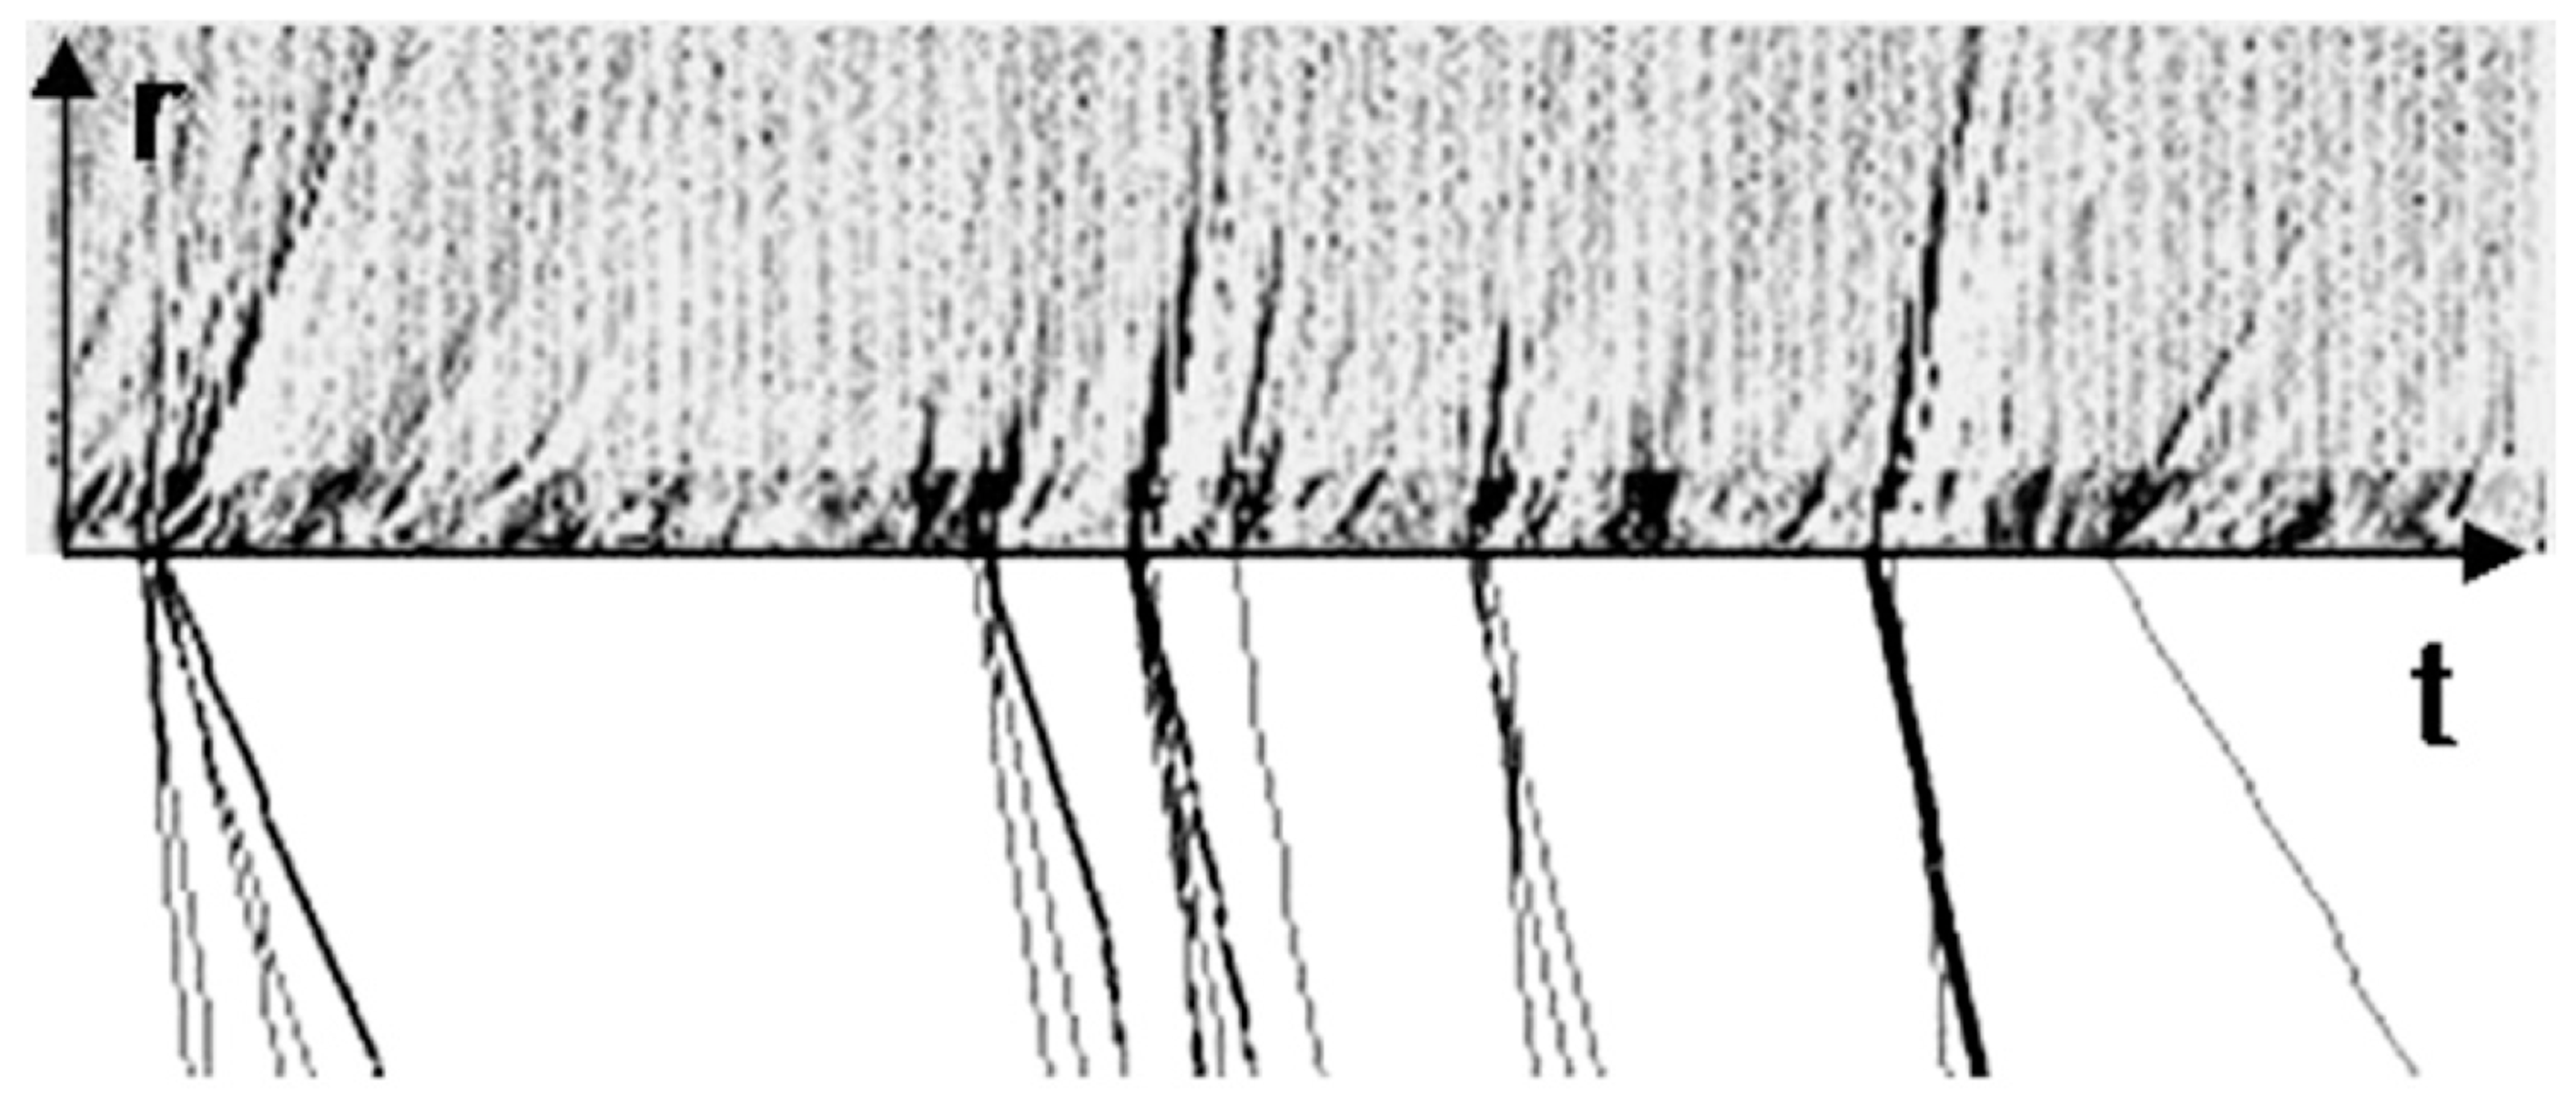
\includegraphics[clip=true, scale=0.25, trim=0 0 0 0]{images/cactusridges.pdf}}
%\label{cactusridges}
%\subfigure[Left: the $(t,\, r)$ slice for a given angle $\theta$, with an example ridge drawn from onset time $t_0$ with duration $\Delta t$ across the field-of-view from $r_{min}$ to $r_{max}$. Right: the corresponding accumulator space $(t_0,\, \Delta t)$ where the ridge will appear as a point with a magnitude corresponding to the ridge intensity. This modified Hough transform is used to threshold the most significant ridges in the slice, automatically detecting the CME in the coronagraph image.]{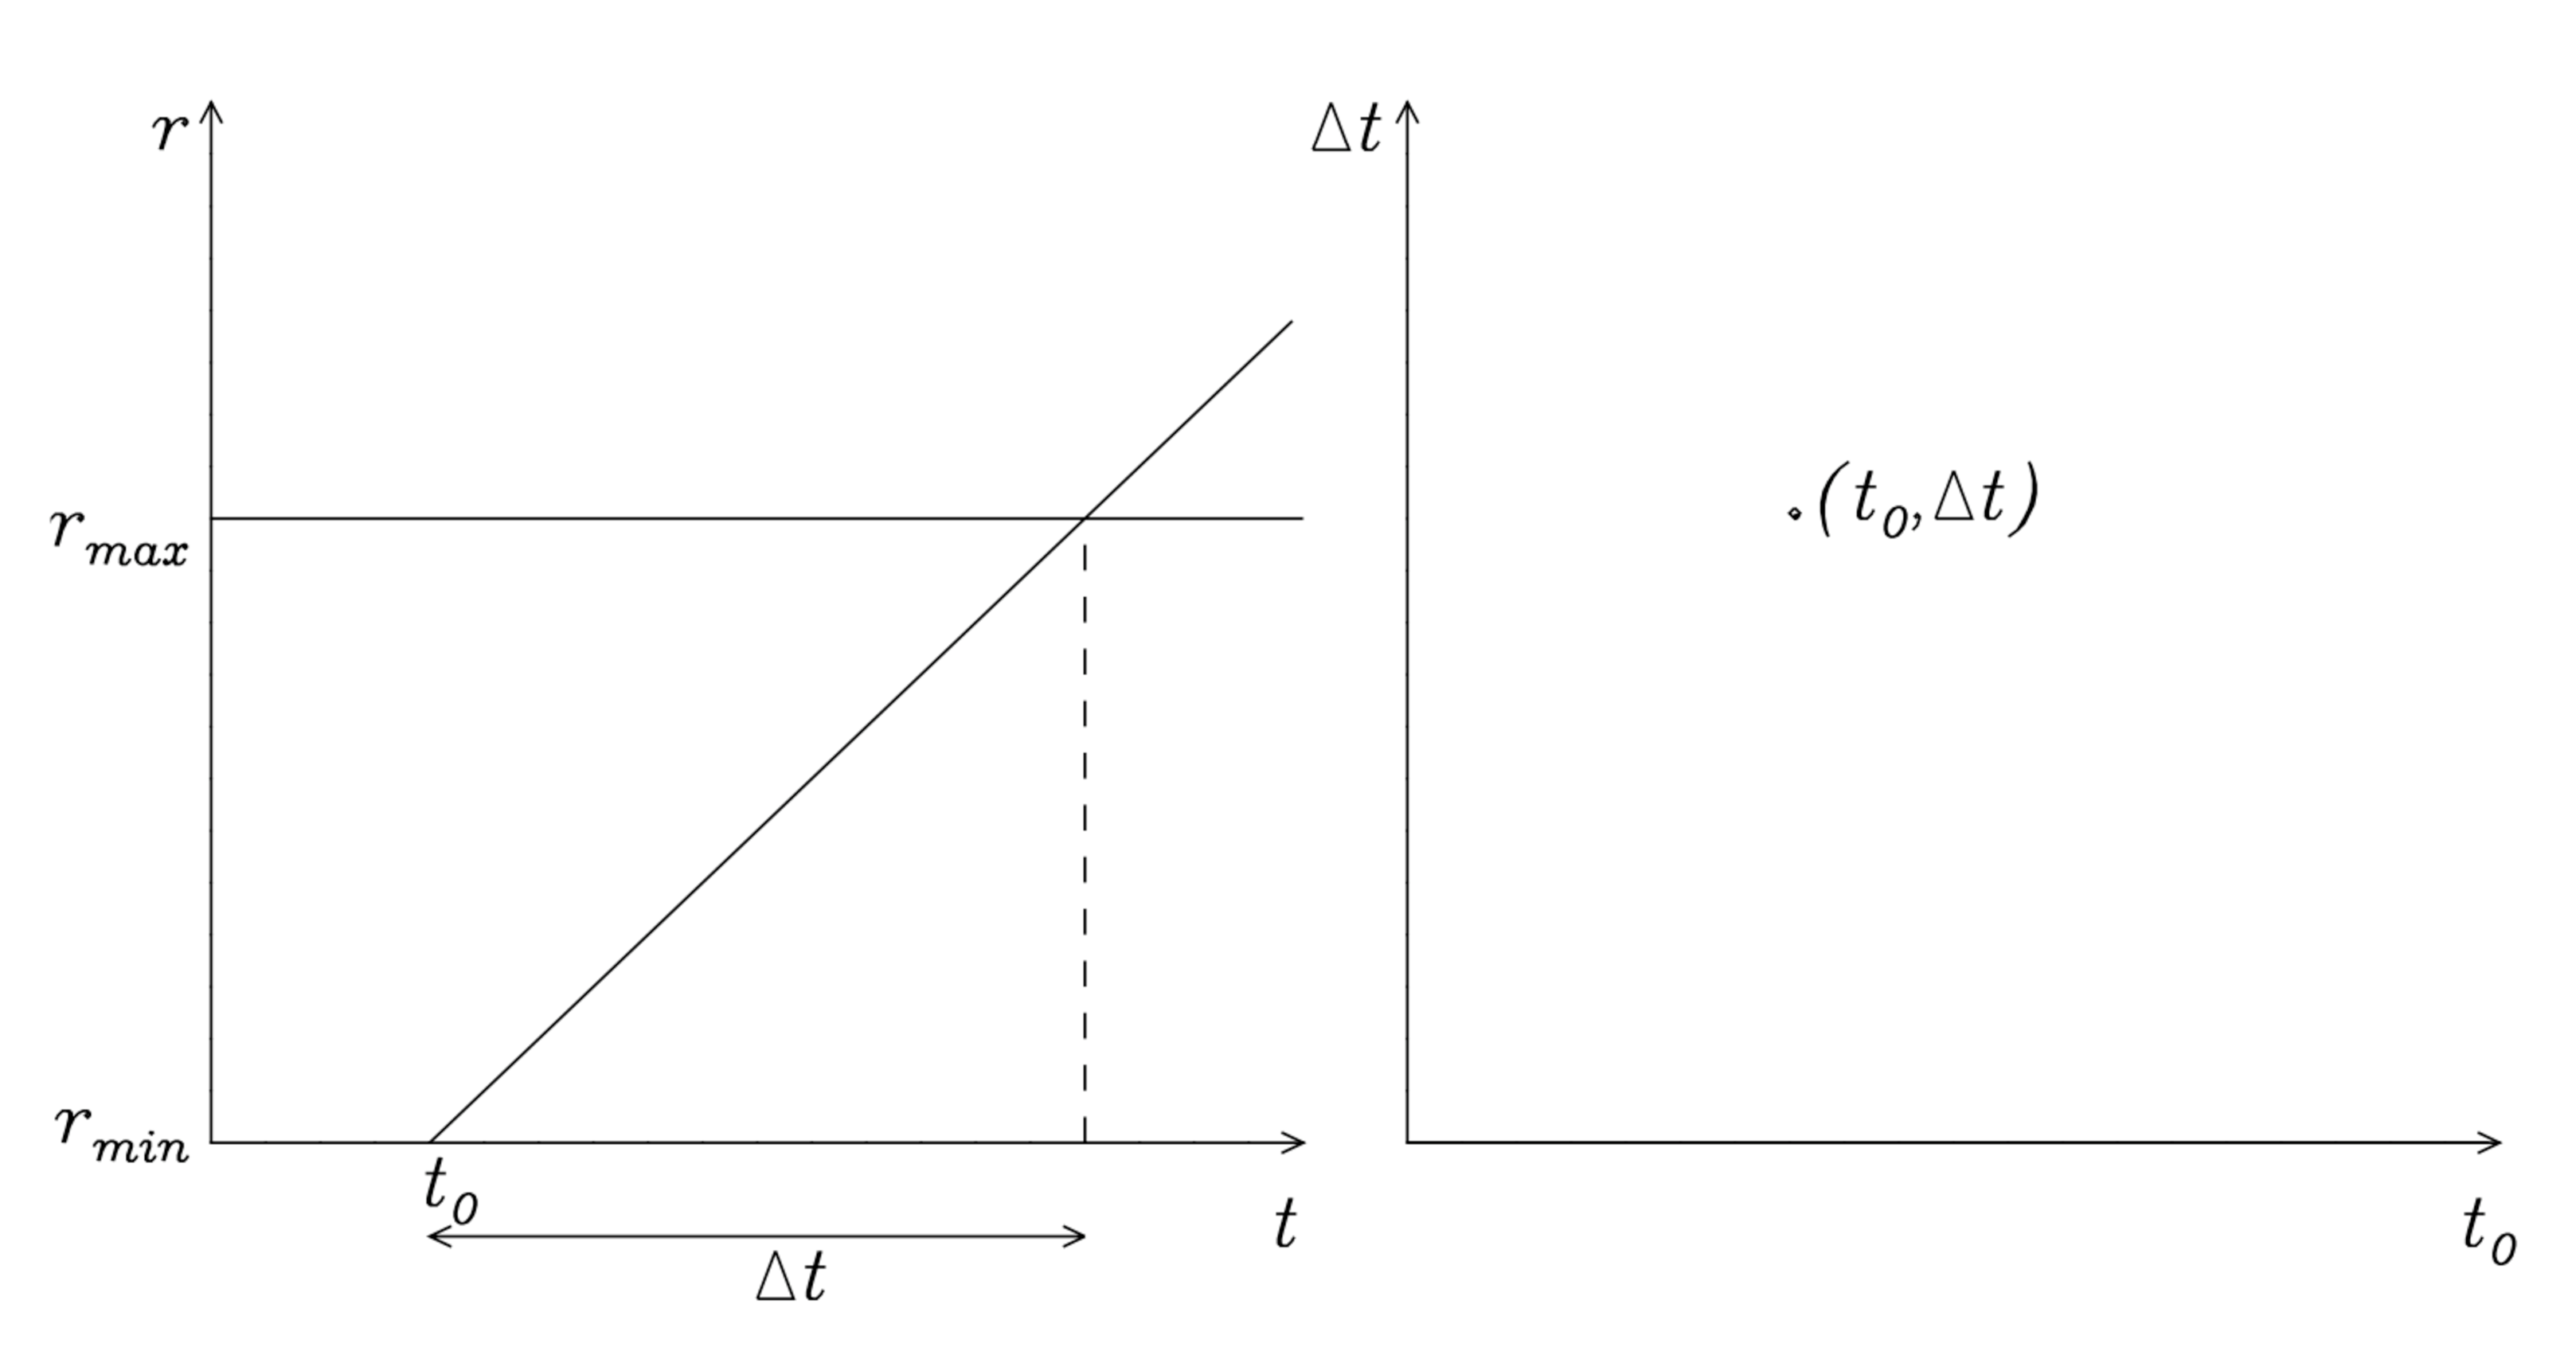
\includegraphics[scale=0.25, clip=true, trim=0 0 0 0]{images/hough.pdf}}
%\caption{The top image (a) shows the detection of ridges in the $(t,\,r)$ stacks of the CACTus catalogue, through the use of the Hough transform detailed in the bottom image (b), reproduced from \citet{2004A&A...425.1097R}.}
%\label{hough}
%\end{figure}

The Computer Aided CME Tracking catalogue \citep[CACTus\footnote{http://sidc.oma.be/cactus/};][]{2004A&A...425.1097R} was the first automated CME detection algorithm, in operation since 2004. It is based upon the detection of CMEs as bright ridges in time-height slices $(t,\, r)$ at each angle $\theta$ around a coronagraph image. The images are preprocessed as standard, then a running-difference technique is applied and each image transformed into Sun-centred polar coordinates $(r,\; \theta)$, rebinned, and the C2 and C3 fields-of-view combined. These are then stacked in time, and for each angle the corresponding $(t,\,r)$ slice undergoes a modified Hough transform for detecting intensity ridges across it. This works by parameterising the $(t,\, r)$ slice by the variables $t_0$ and $\Delta t$, corresponding to the coordinate intersection point with the time axis, and the distance along the time axis respectively (together called the accumulator space; see Figure~\ref{hough}). So the equation of a line corresponding to an intensity ridge in the slice is given by:
\begin{equation}
r \; = \; \frac{r_{max}-r_{min}}{\Delta t} (t-t_0) + r_{min}
\end{equation}
Thresholding the most significant ridges in the resultant accumulator space filters out the progression of CMEs, with the variables for each ridge characterised by onset time $t_R$, the velocity $v_R \; \left( \sim \frac{1}{\Delta t} \right)$, for angle $\theta_R$, to give a characteristic variable $I_R=\left(v_R,\, \theta_R,\, t_R \right)$. A 3D scatter plot $(v,\, \theta,\, t)$ of all detected ridges $I_R$ is then integrated along the $v$-direction to identify clusters in the resulting $(\theta,\, t)$ map which illustrates the angular span and duration time of the detected CMEs in the coronagraph data. A median velocity across the angular span is quoted as the CME speed.
\newline
\indent The running-difference cadence, the ridge intensity threshold, and the imposed limit on how many frames a CME may exist (and indeed the definition of a CME) all affect how successful the detection can be. However, \citet{2004A&A...425.1097R} show the algorithm to be robust in reproducing well the detections of a human user by direct comparison with the CDAW catalogue. The main drawback of the CACTus catalogue for studying CMEs is the imposed zero acceleration of the detection algorithm, since the Hough transform thresholds the ridges as straight lines whose slopes provide a constant velocity. The velocity itself may also be underestimated since it is a median across the span of the CME. The angular spans are possibly over-estimated since side outflows in the images are enhanced by the running-difference and may also include streamer deflections. It is also difficult to distinguish when one CME has fully progressed from the field-of-view and another CME has entered it, so in some cases trailing portions of a CME are detected as separate events.

\subsubsection{SEEDS}

\begin{figure}[!ht]
\centerline{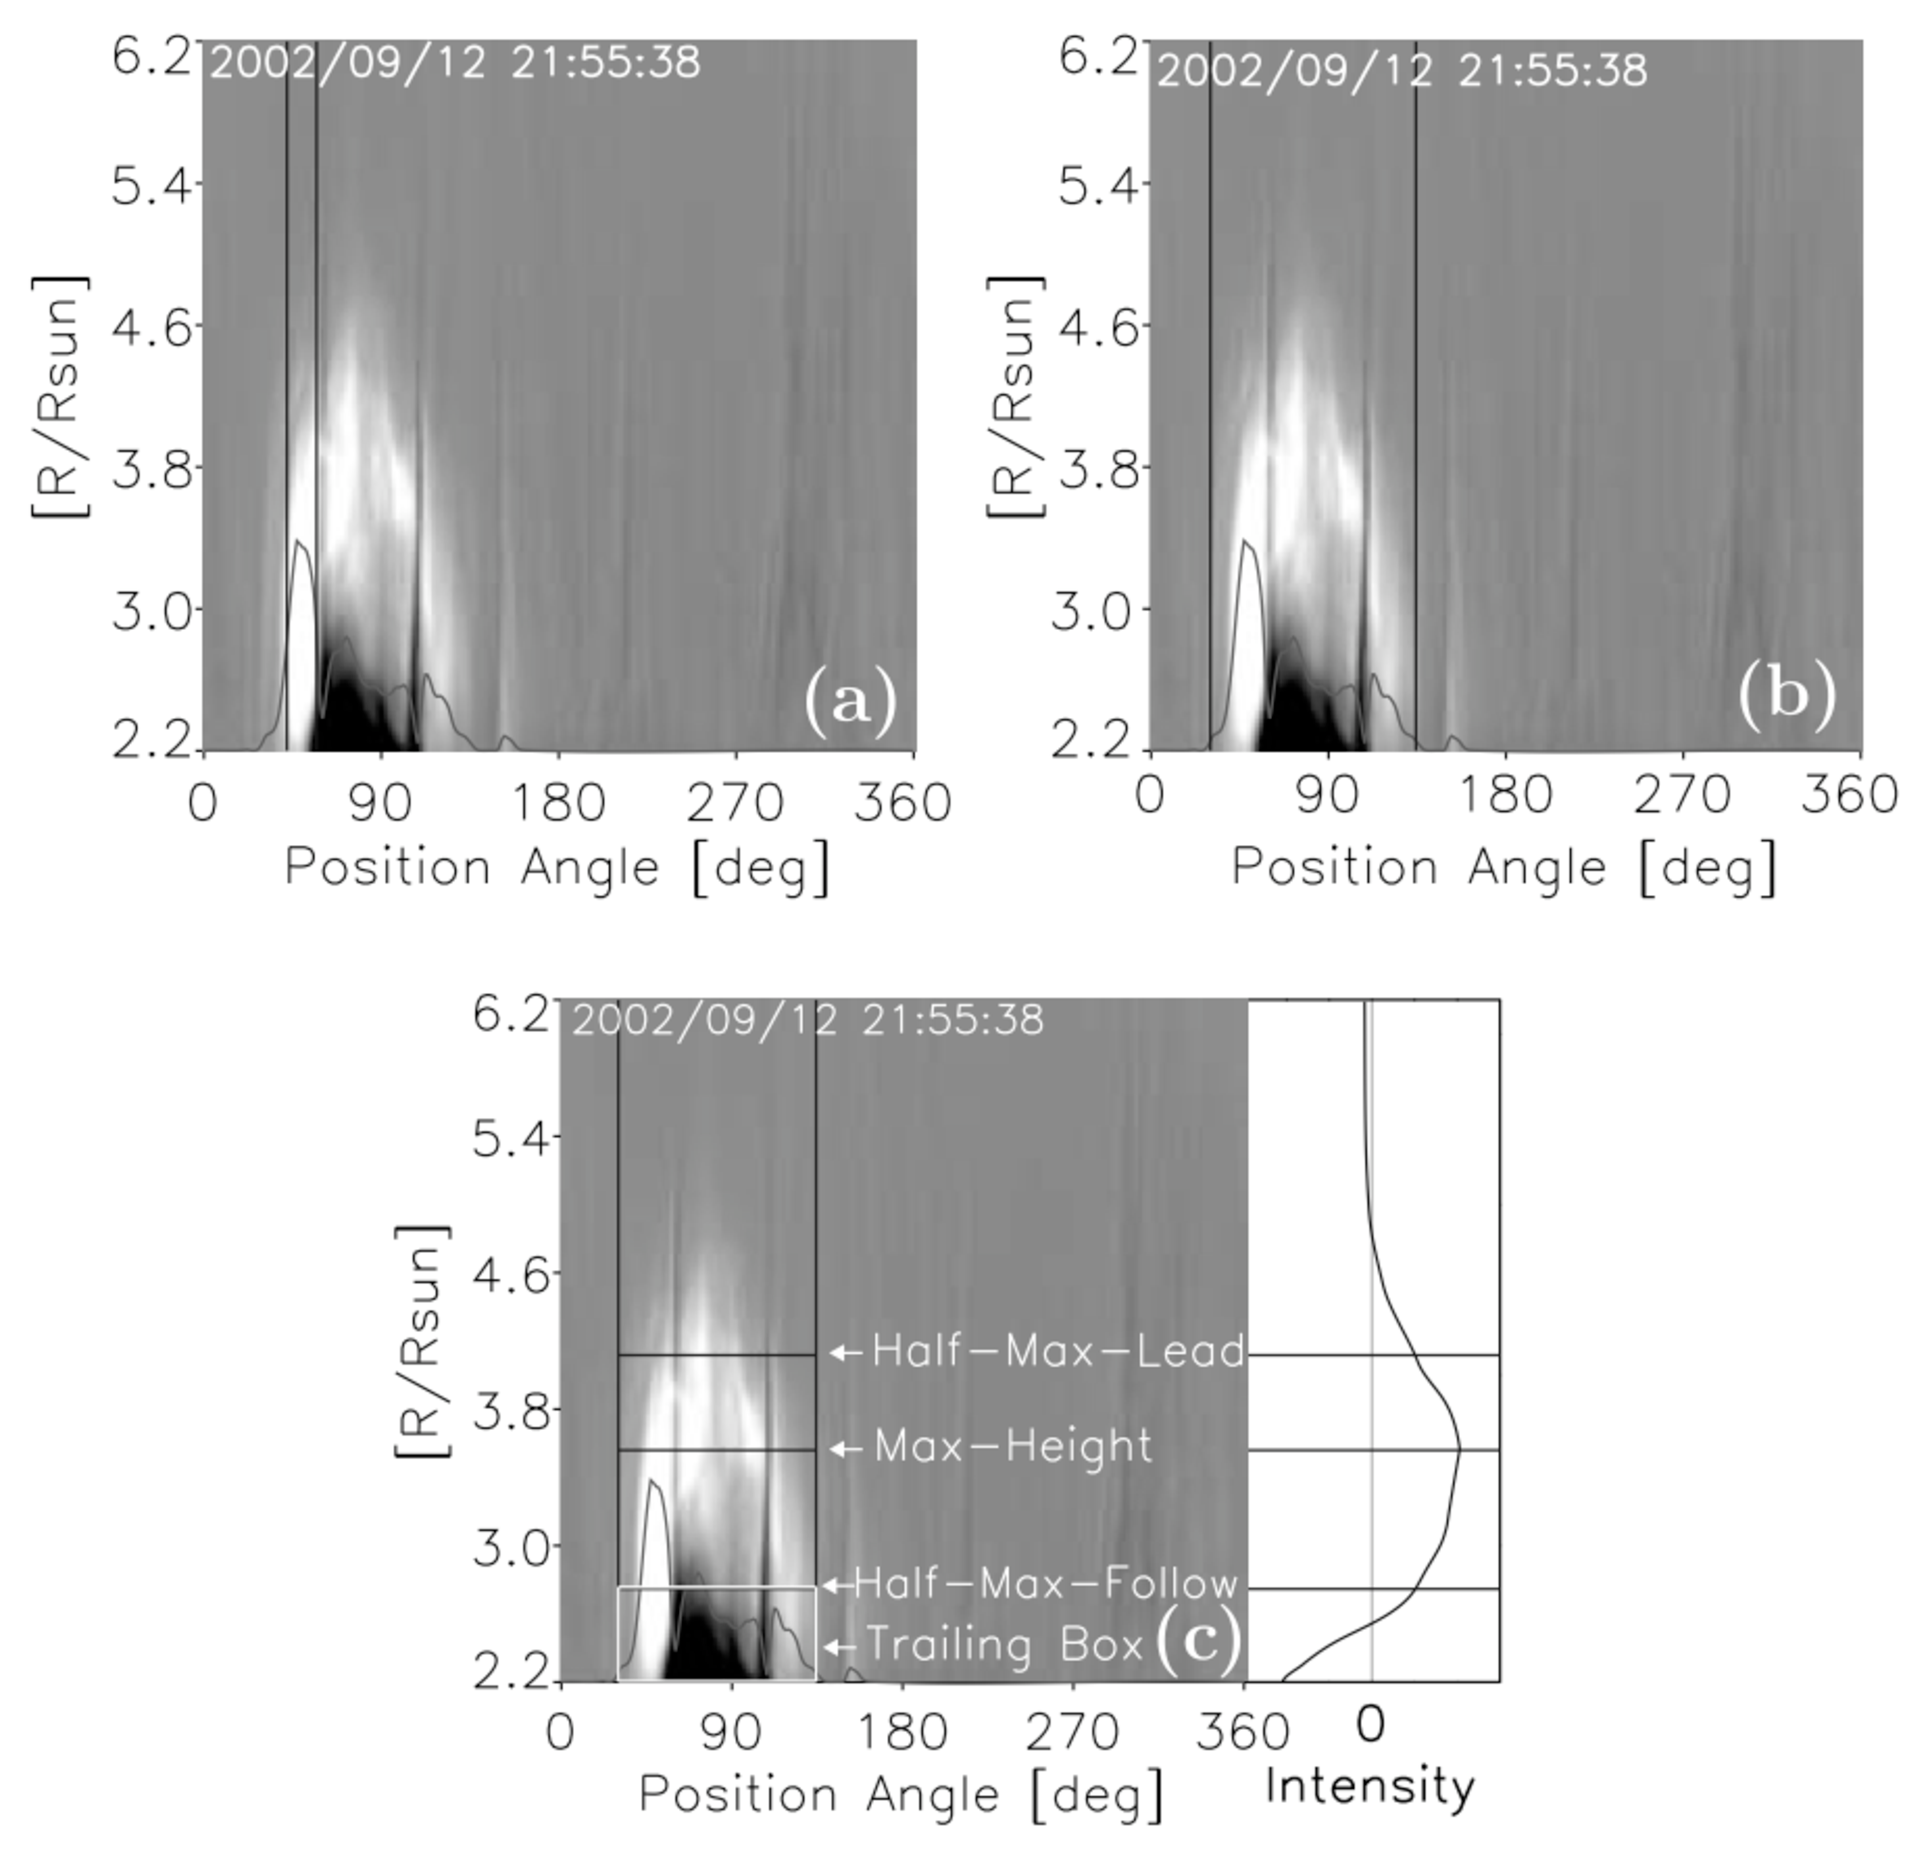
\includegraphics[scale=0.45, clip=true, trim=0 0 0 0]{images/SEEDS.pdf}}
\caption{Example of the SEEDS CME detection and height determination, reproduced from \citet{2008SoPh..248..485O}. ({\bf a}) shows the running-difference image unwrapped into Sun-centre polar coordinates, showing a CME observed by LASCO/C2 on 12 September 2002. The black line distribution across the image represents the positive value intensity count along each angle, and the two vertical black lines mark the angular span at one standard deviation above the mean intensity. ({\bf b}) shows the new angular span following the region growing technique. ({\bf c}) shows the intensity within the angular span averaged across heights, and the `Half-Max-Lead' is taken as the CME height in the image.}
\label{seeds}
\end{figure}

The Solar Eruptive Event Detection System \citep[SEEDS\footnote{http://spaceweather.gmu.edu/seeds/};][]{2008SoPh..248..485O} is an automated CME detection algorithm for tracking an intensity thresholded CME front in running-difference images from LASCO/C2. The images are preprocessed as standard, unwrapped into Sun-centred polar coordinates $(r,\; \theta)$, and a normalised running-difference technique is applied using the following equation:
\begin{equation}
u_i \; = \; \left[ n_i - n_{i-1} \left( \frac{\bar{n}_i}{\bar{n}_{i-1}} \right) \right] \frac{\alpha}{\Delta t}
\end{equation}
where $u_i$ is the running-difference image, $\bar{n}$ is the mean of the pixels in the entire field-of-view of the image $n$, $\Delta t$ is the time difference between images (in minutes), $\alpha$ is a constant set to approximately the smallest time difference ($\Delta t$) between any image pair, where $i$ is the current image and $i-1$ the preceding image. This normalised difference ensures that the mean of the new image ($u_i$) will effectively be zero.
\newline
\indent The pixel intensities (positive values only) are then summed along angles and thresholded at a certain number of standard deviations above the mean intensity: $\mu+N\sigma$ (cf. Equation~\ref{eqn:threshold}) as in Figure~\ref{seeds}a. This determines the `core angles' of the CME, and a region growing technique based on a secondary threshold of intensities in the rest of the image is applied to open the angular span to include the full CME (Figure~\ref{seeds}b). Issues arise when streamer deflections occur that will offset the region growing technique and overestimate the CME angular width. An intensity average across the angles within the span of the CME is then determined, and where the forward portion of this intensity profile equals half its maximum value is taken as the CME height (Figure~\ref{seeds}c). The velocity and acceleration are determined from the heights through consecutive images and these results are output with the CME position angle and angular width in the SEEDS catalogue.
\newline
\indent Along with the issues of streamer deflections and the tracking being limited to C2 images, the choice of the `Half-Max-Lead' as the CME height is dependant on the overall CME brightness, and thus any brightness changes as the CME propagates will affect this measurement. This would add to the error on the height-time profile which, along with the error in time as a result of the running-difference technique, makes it difficult to accurately determine the velocity and acceleration.

\subsubsection{ARTEMIS}

The Automatic Recognition of Transient Events and Marseille Inventory from Synoptic maps \citep[ARTEMIS\footnote{http://www.oamp.fr/lasco/};][]{2009SoPh..257..125B} is an automated CME detection algorithm that works by identifying signatures of transients in synoptic maps. These maps are generated as $(t,\, \theta)$ slices for specific heights $r$ in the coronagraph images of LASCO/C2. The images are prepared through the standard preprocessing steps. Then at a specific height (e.g., $r=3$~R$_{\odot}$) the intensity is plotted across all angles $\theta$ for each image through time $t$ with transient events appearing as vertical streaks through the more persistent streamer intensities (Figure~\ref{artemis}). A method of image filtering and intensity thresholding is applied to distinguish the streaks in the synoptic map, and image segmentation then discards small features and closes off regions-of-interest (ROIs) to produce a binary map of the streaks. Specific parameters of these streaks are also computed, such as their total radiances, areas and centres of gravity. Merging with high-level knowledge helps to associate ROIs of the same CME if three criteria are met: the difference between the $x$-coordinates of the centres of two ROIs differs by less than two pixels; the difference between the $y$-coordinates of their centres differs by less than 60 pixels (corresponding to a 60$^{\circ}$ angular span); and the ratio of their radiances calculated at their centres (on the original synoptic map) ranges from 0.25 to 4. The result is a binary CME detection map in $(t,\, \theta)$ space for different heights in the corona: 3, 3.5, 4, 4.5, 5 and 5.5 R$_{\odot}$.

\begin{figure}[!ht]
\centerline{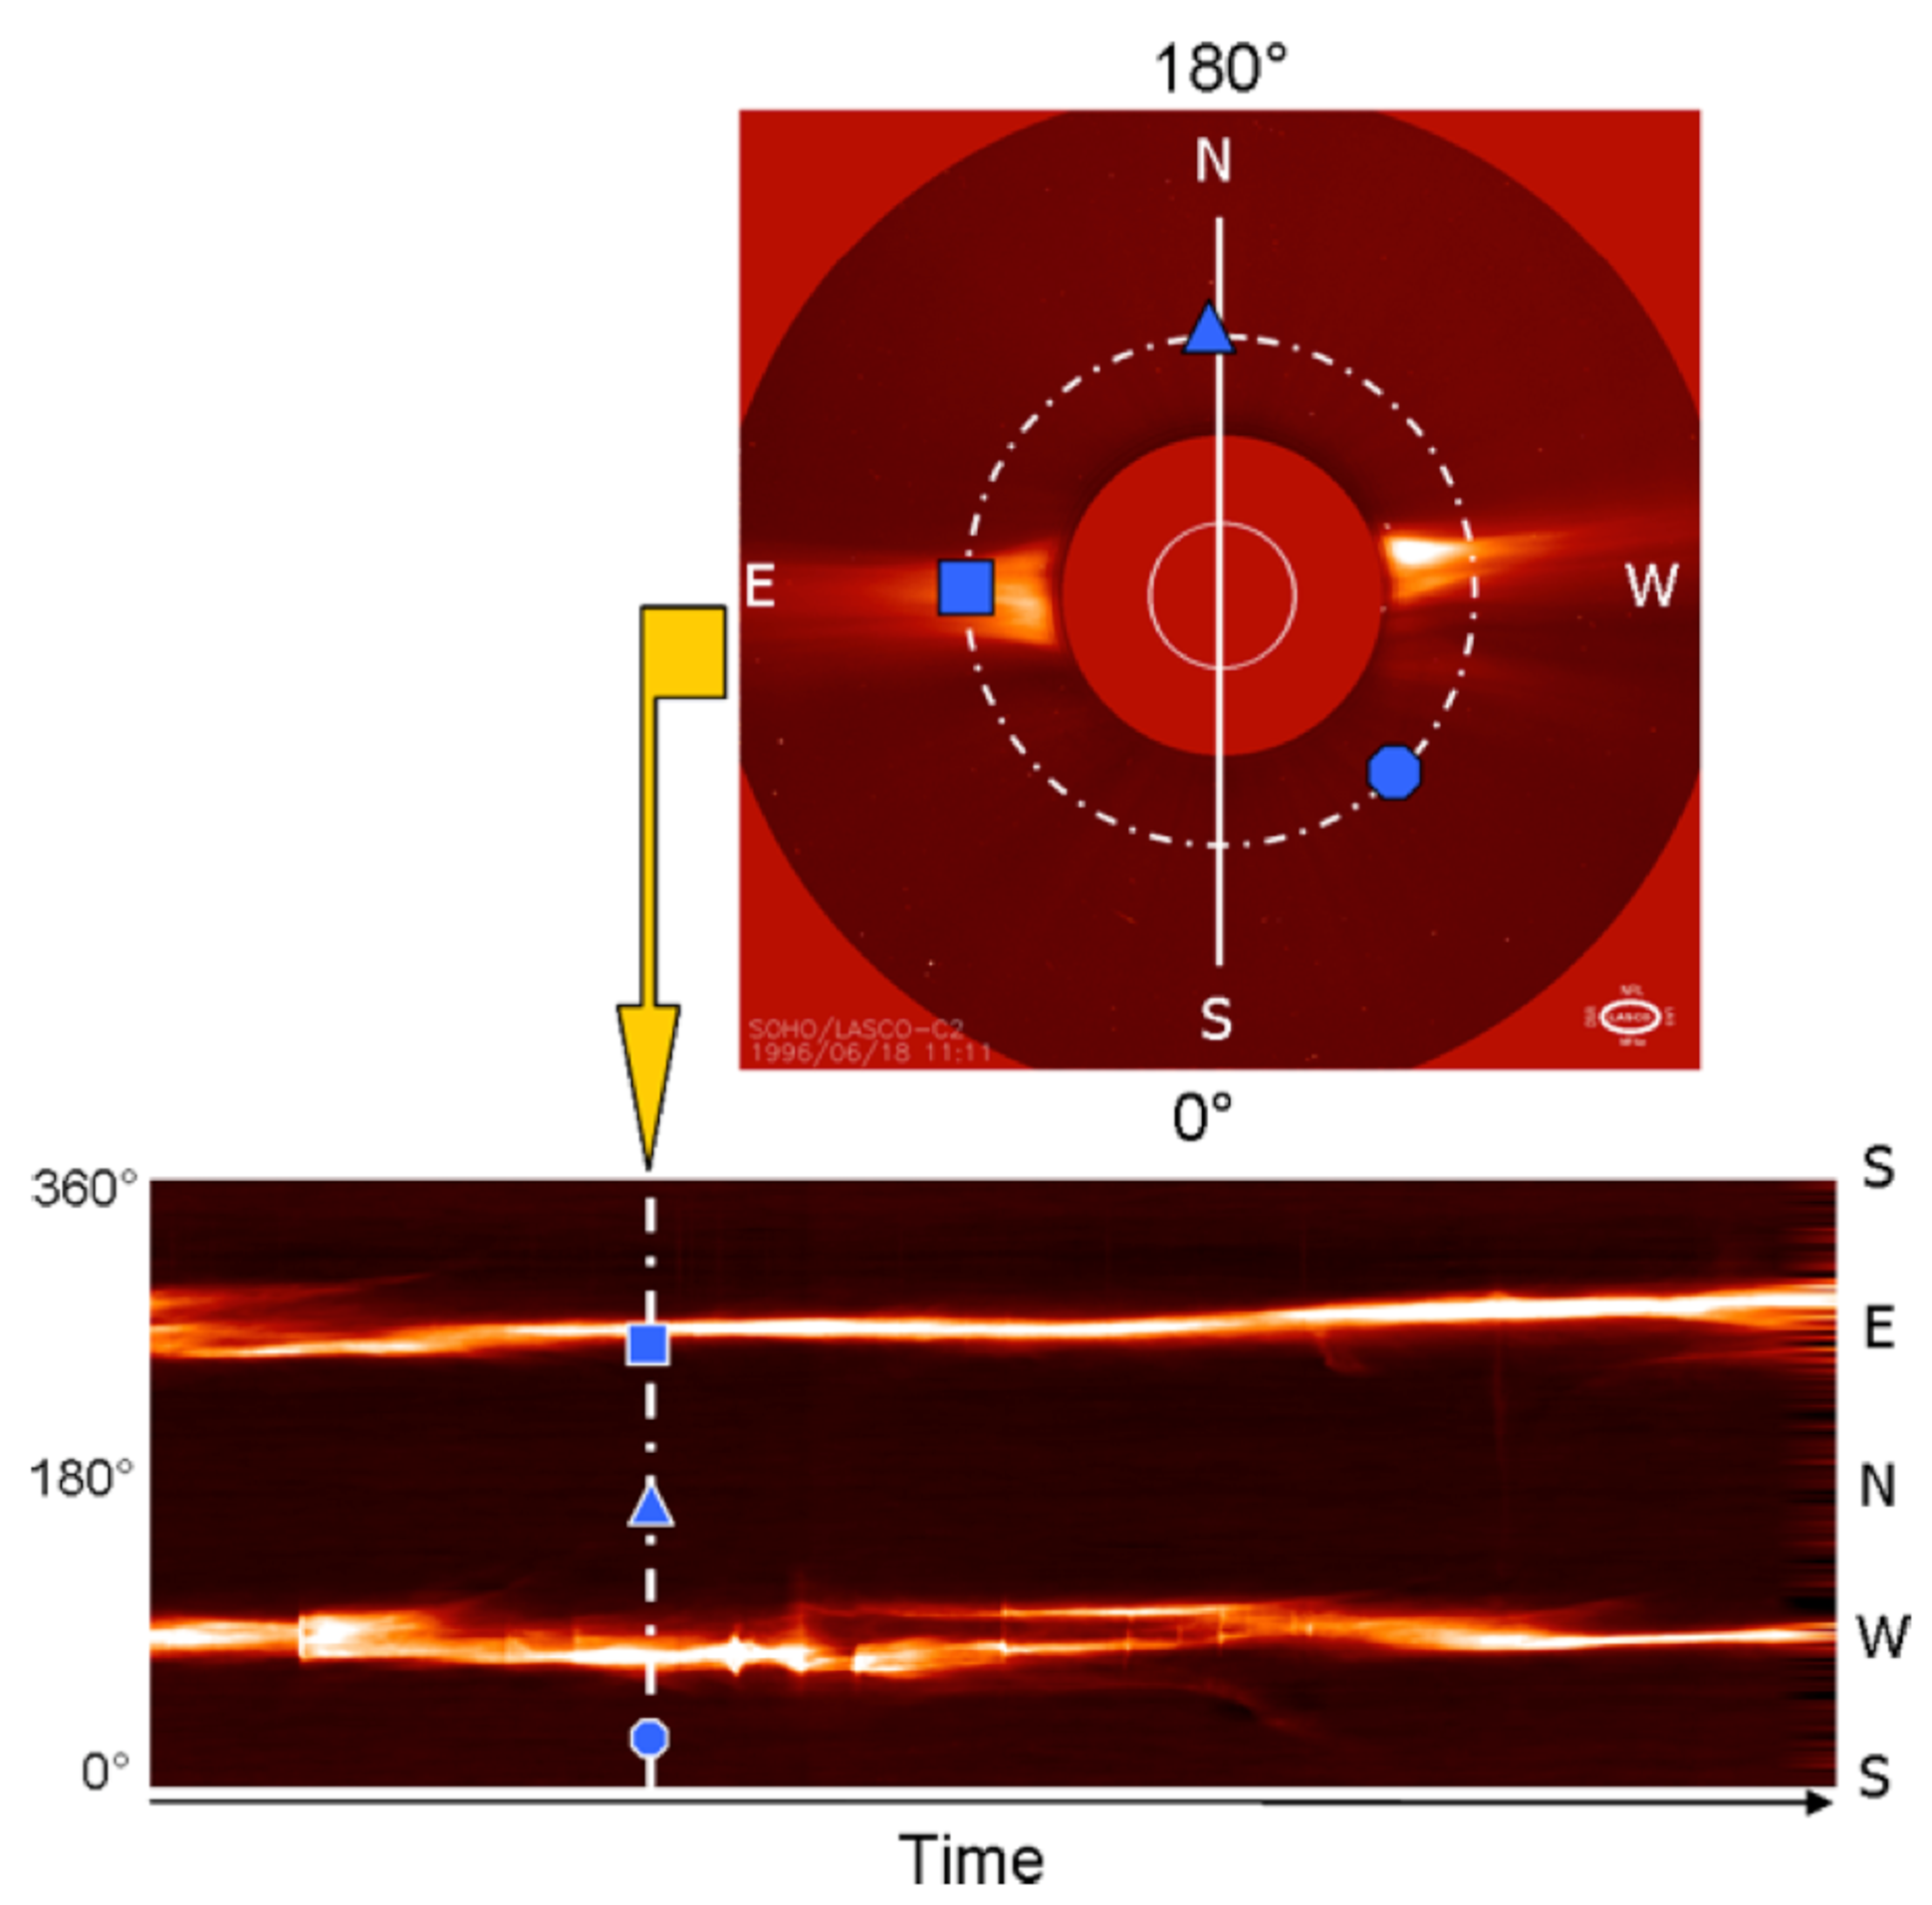
\includegraphics[scale=0.43, clip=true, trim=0 0 0 0]{images/ARTEMIS.pdf}}
\caption{An example of how the synoptic maps are generated for the ARTEMIS catalogue, reproduced from \citet{2009SoPh..257..125B}. At a chosen height in the coronagraph image an annulus is unwrapped (indicated with the dashed line and blue square, circle and triangle) and these are then stacked together to illustrate how the intensity at that height changes through time. Vertical streaks represent transient events occurring on smaller time-scales than the more persistent streamers in the images.}
\label{artemis}
\end{figure}

With the CME detections in place, estimates of the velocity may be made. A first estimate is taken by testing a range of constant velocities 50\,--\,2,000~km~s$^{-1}$ to determine which best matches the shifting of the CME detection in synoptic maps at subsequent heights through the corona. The binary maps are shifted by an amount corresponding to velocity steps of 10~km~s$^{-1}$, such that the one which provides the maximum pixel value (with a minimum limit of 3) indicates the best velocity estimate of the event. A second estimate is taken by cross-correlating the detected CME ROIs on the original synoptic maps at 3~R$_{\odot}$ and 5.5~R$_{\odot}$ and inspecting the intensity shift in time (pixel shift in $x$-direction) to obtain the velocity estimate. A third estimate is taken by similar cross-correlation but specifically on each individual line of the ROIs to obtain a distribution of velocities across the angular span of the CME, the median of which is taken as the actual velocity. \citet{2009SoPh..257..125B} compare histograms of the three different velocity estimates for the ARTEMIS CME detections over a twelve year interval and find that, globally, the three estimates are highly consistent with each other.

ARTEMIS is limited to the C2 field-of-view and it provides kinematics only in the 3\,--\,5.5~R$_{\odot}$ range. The velocity determinations themselves are not specific to either the CME front nor any other identifiable feature, and carry all the inaccuracies resulting from the image rebinning, intensity averaging, filtering and segmentation techniques in generating the final detection masks.
\par
Due to the drawbacks of each of the catalogues above, the motivation exists to study the kinematics and morphology of CMEs with as great an accuracy as possible in order to better compare with theory. To this end we outline below our application of multiscale analysis to remove small scale noise/features and enhance the larger scale CME in single coronagraph frames, allowing the CME front edges to be detected and a geometrical characterisation applied to study its propagation with increased accuracy for deriving the kinematics and morphology.

\subsection{Multiscale Filtering}

In this section a new multiscale method of analysing CMEs is described. The use of multiscale methods in astrophysics have proven effective at denoising spectra and images \citep{1995A&AS..112..179M, 1997A&AS..124..579F}, analysing solar active region evolution \citep{2008SoPh..248..311H}, and enhancing solar coronal images \citep{2003A&A...398.1185S, 2008ApJ...674.1201S}.  A particular application of multiscale decompositions uses high and low pass filters convolved with the image data to exploit the multiscale nature of the CME \citep{2008SoPh..248..457Y}. This highlights its intensity against the background corona as it propagates through the field-of-view, while neglecting small scale features (essentially denoising the data). It also leads to the use of non-maxima suppression to trace the edges in the CME images, and  \citet{2008SoPh..248..457Y} show the power of multiscale methods over previous edge detectors such as Roberts \citep{1975CGIP....4..248D} and Sobel \citep{1973pcsa.book.....D}. With these methods for defining the front of the CME we can characterise its kinematics (position, velocity, acceleration) and morphology (width, orientation) in coronagraph images. Multiscale analysis also has the benefit of working on independent images without any need for differencing, so the temporal errors involved are on the order of the exposure time of the instrument ($\sim$ a few seconds). 

The fundamental idea behind wavelet analysis is to highlight details apparent on different scales within the data. An example of this is the suppression of noise in images, which tends to occur only on the smallest scales. Wavelets have benefits over previous methods (e.g., Fourier transforms) because they are localised in space and are easily dilated and translated in order to operate on multiple scales, the basic equation being:
\begin{equation}
\psi_{a,b}(t)\,=\, \frac{1}{\sqrt{b}} \, \psi (\frac{t-a}{b})
\end{equation}
where $a$ and $b$ represent the shifting (translation) and scaling (dilation) of the mother wavelet $\psi$ which can take several forms depending on the required use. 

We explore a method of multiscale decomposition in 2D through the use of low and high pass filters; using a discrete approximation of a Gaussian, $\theta$, and its derivative, $\psi$, respectively \citep{2003A&A...398.1185S}. Since $\theta(x,y)$ is separable, i.e. $\theta(x,y)=\theta(x)\theta(y)$, we can write the wavelets as the first derivative of the smoothing function:
\begin{eqnarray}
\psi_{x}^{s}(x,y)\,&=\, s^{-2} \frac{\partial \theta(s^{-1}x)}{\partial x}\theta(s^{-1}y) \\
\psi_{y}^{s}(x,y)\,&=\, s^{-2} \theta(s^{-1}x)\frac{\partial \theta(s^{-1}y)}{\partial y}
\end{eqnarray}
where $s$ is the dyadic scale factor such that $s=2^j$ where $j=1,2,3,...,J$. Successive convolutions of an image with the filters produces the scales of decomposition, with the high-pass filtering providing the wavelet transform of image $I(x,y)$ in each direction:
\begin{eqnarray}
W_{x}^{s}I \,&\equiv\, W_{x}^s I(x,y)\,=\,\psi_{x}^s (x,y)*I(x,y) \\
W_{y}^{s}I \,&\equiv\, W_{y}^s I(x,y)\,=\,\psi_{y}^s (x,y)*I(x,y)
\end{eqnarray}

\begin{figure}[!ht]
\centerline{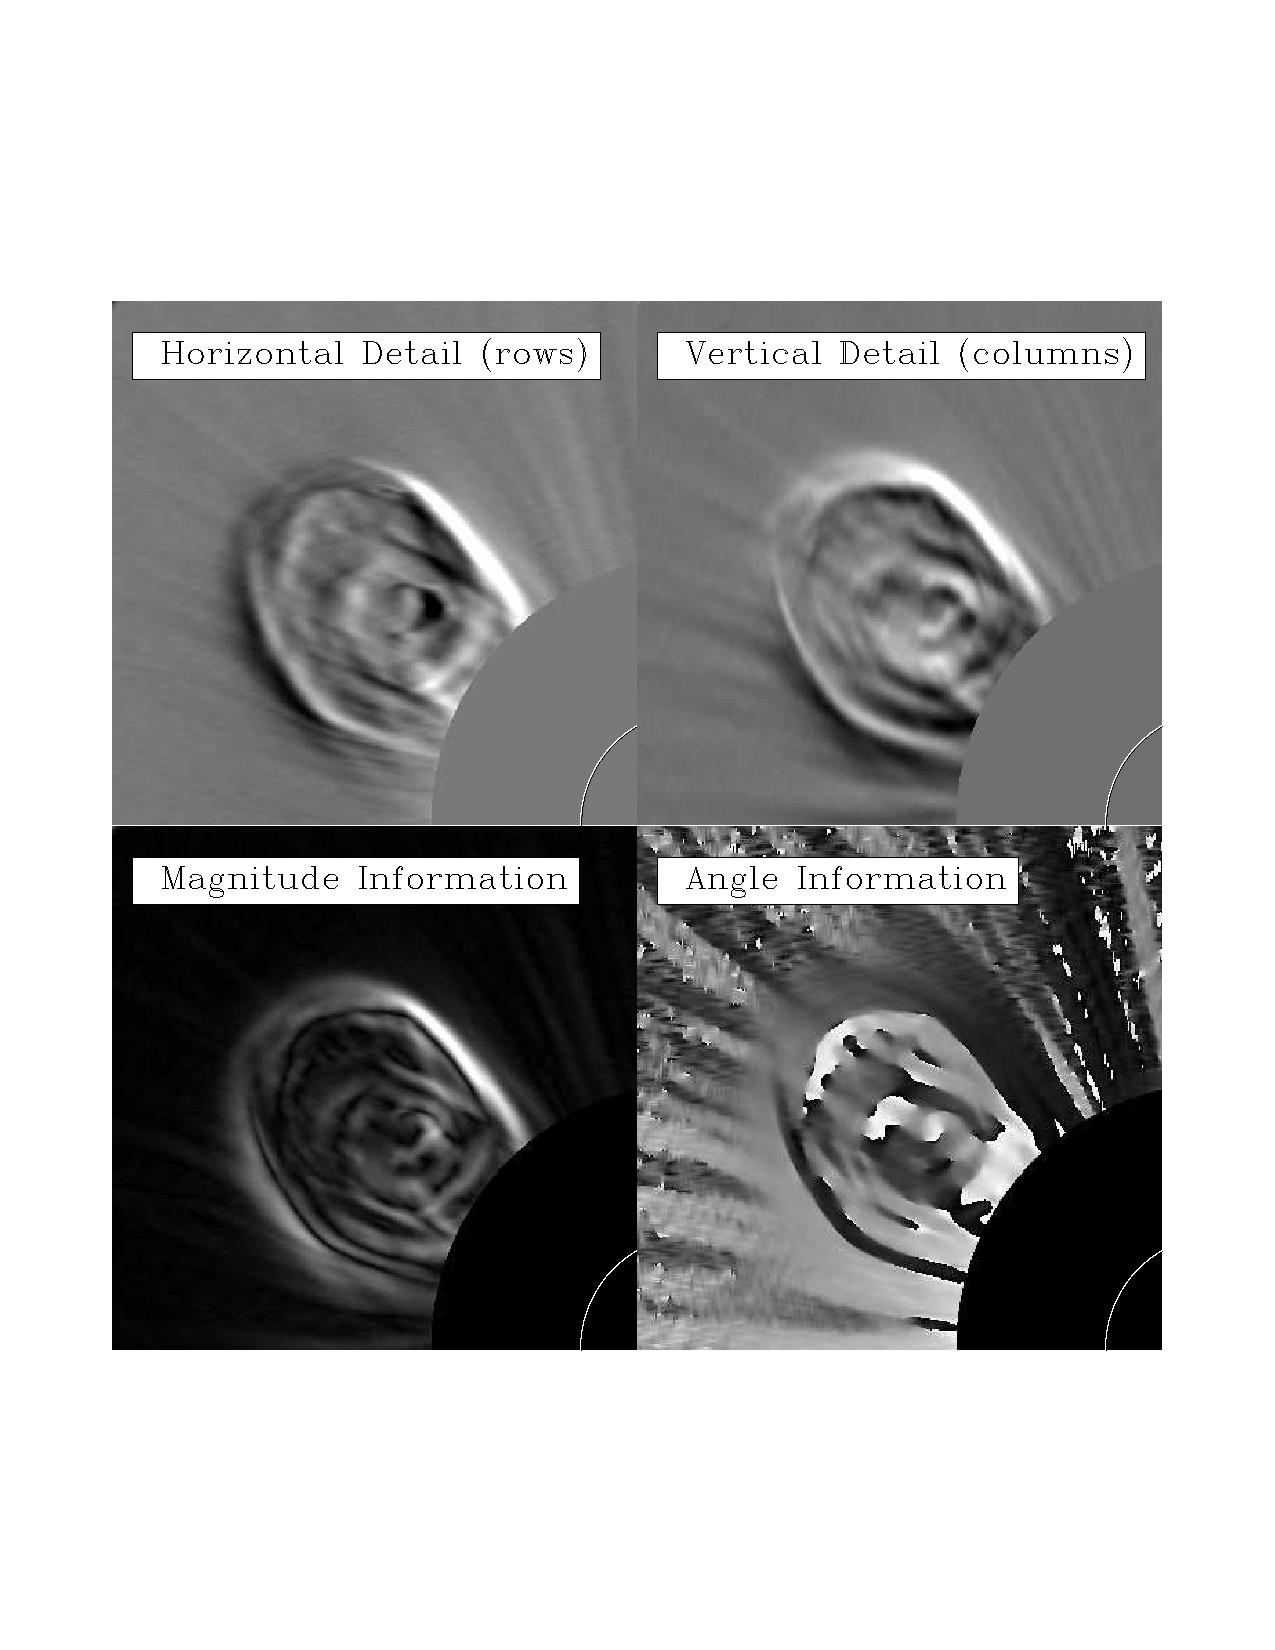
\includegraphics[scale=0.8, clip=true, trim=0 130 0 150]{images/canny_images.pdf}}
\caption{Top left, the horizontal detail, and top right, the vertical detail from the high-pass filtering at one scale of the multiscale decomposition (called the rows and columns respectively). Bottom left, the corresponding magnitude (edge strength) and bottom right, the angle information (0 -- 360$^{\circ}$) taken from the gradient space, for a CME observed in LASCO/C2 on 1 April 2004 \citep{2009A&A...495..325B}.}
\label{decomp}
\end{figure}

Akin to a Canny edge detector \citep{2008SoPh..248..457Y}, these horizontal and vertical wavelet coefficients are combined to form the gradient space, $\Gamma^s(x,y)$, for each scale: 
\begin{equation}
\Gamma^s (x,y)\, = \,\left[W_{x}^s I,~W_{y}^s I \right]
\end{equation}
The gradient information has an angular component $\alpha$ and a magnitude (edge strength) $M$:
\begin{eqnarray}
\alpha^s(x,y) \, &= \, tan^{-1}\left( W_{y}^s I~/~W_{x}^s I \right) \\
M^s(x,y) \, &= \, \sqrt{ ( W_{x}^s I ) ^2 + ( W_{y}^s I ) ^2 }
\end{eqnarray}
The resultant horizontal and vertical detail coefficients, and the magnitude and angular information are illustrated in Figure~\ref{decomp}.
%\begin{figure}[!ht]
%\centering
%\subfigure[00:40 UT]
%{
%	\label{arrow1}
%	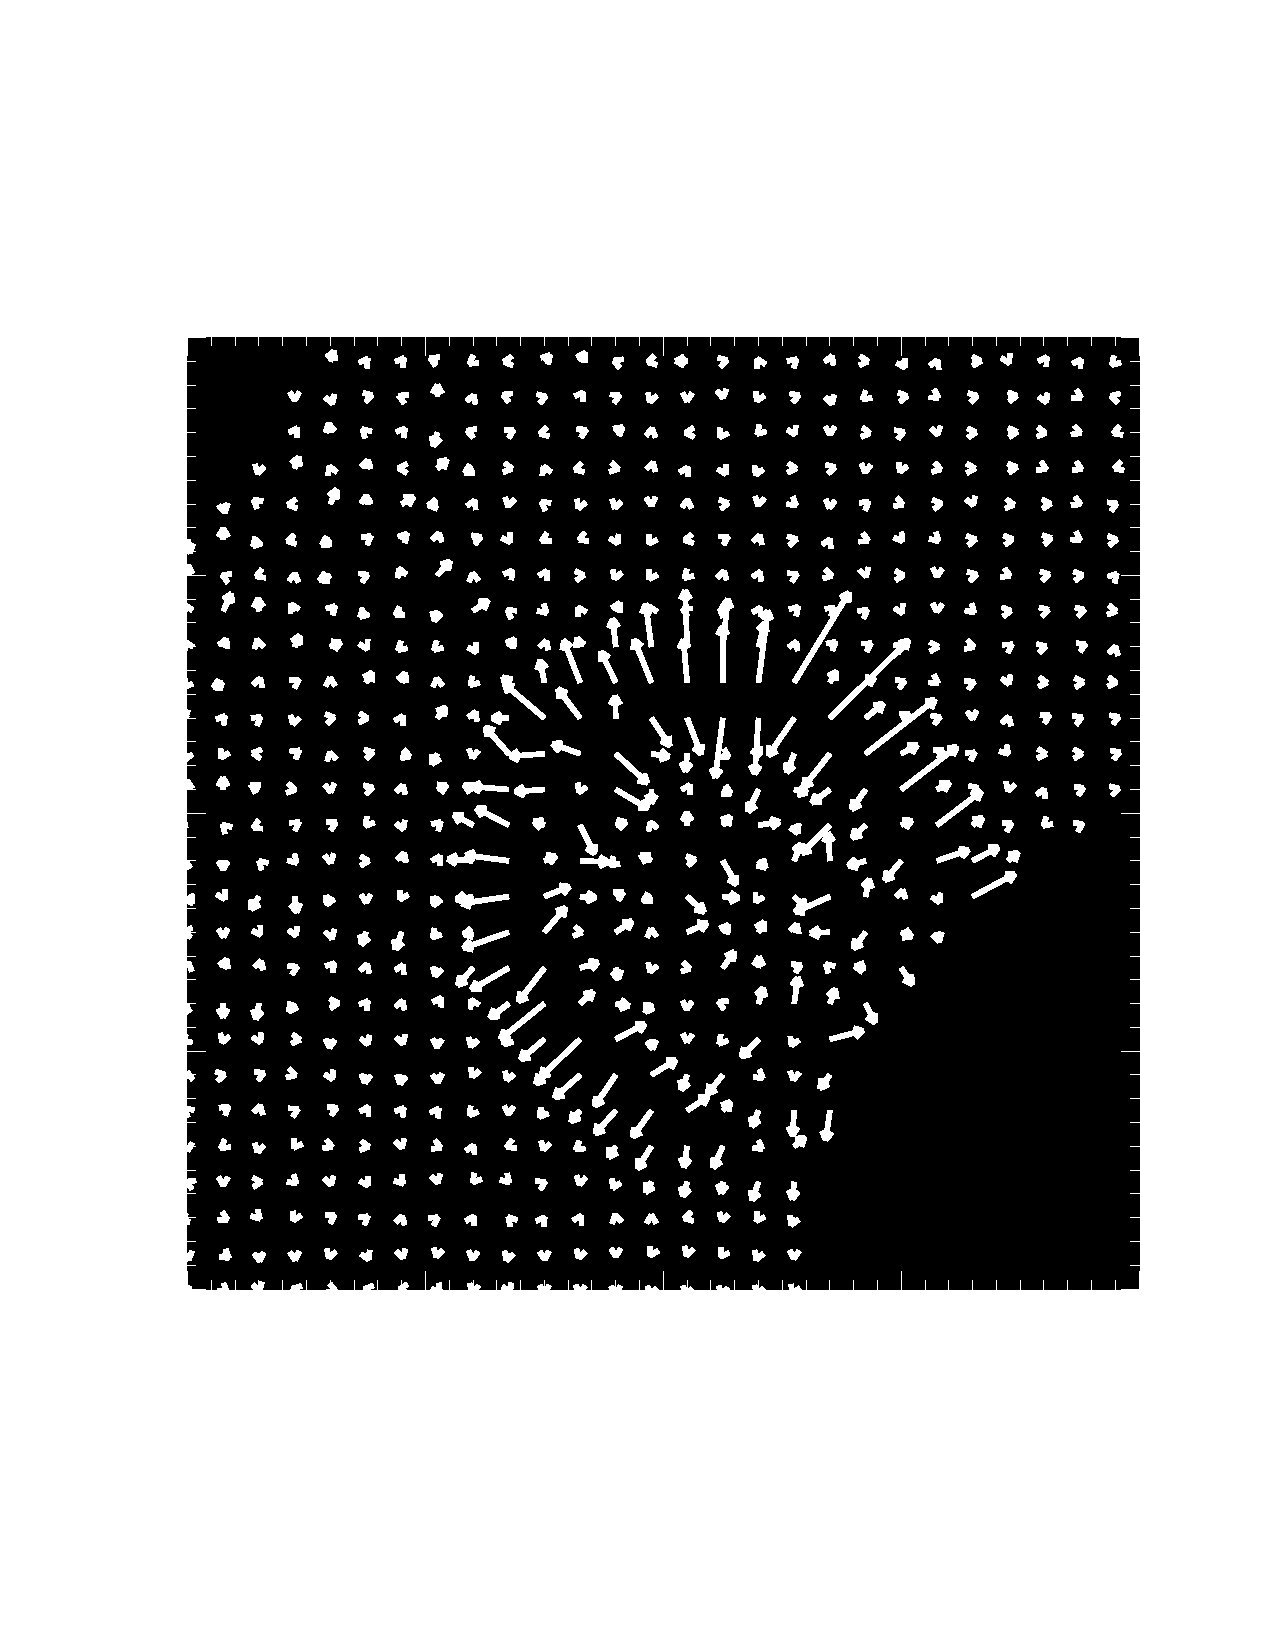
\includegraphics[scale=0.35, trim=105 130 0 130]{images/arrow1.pdf}		
%}
%\vspace{0cm}
%\subfigure[01:00 UT]
%{
%	\label{arrow2}
%	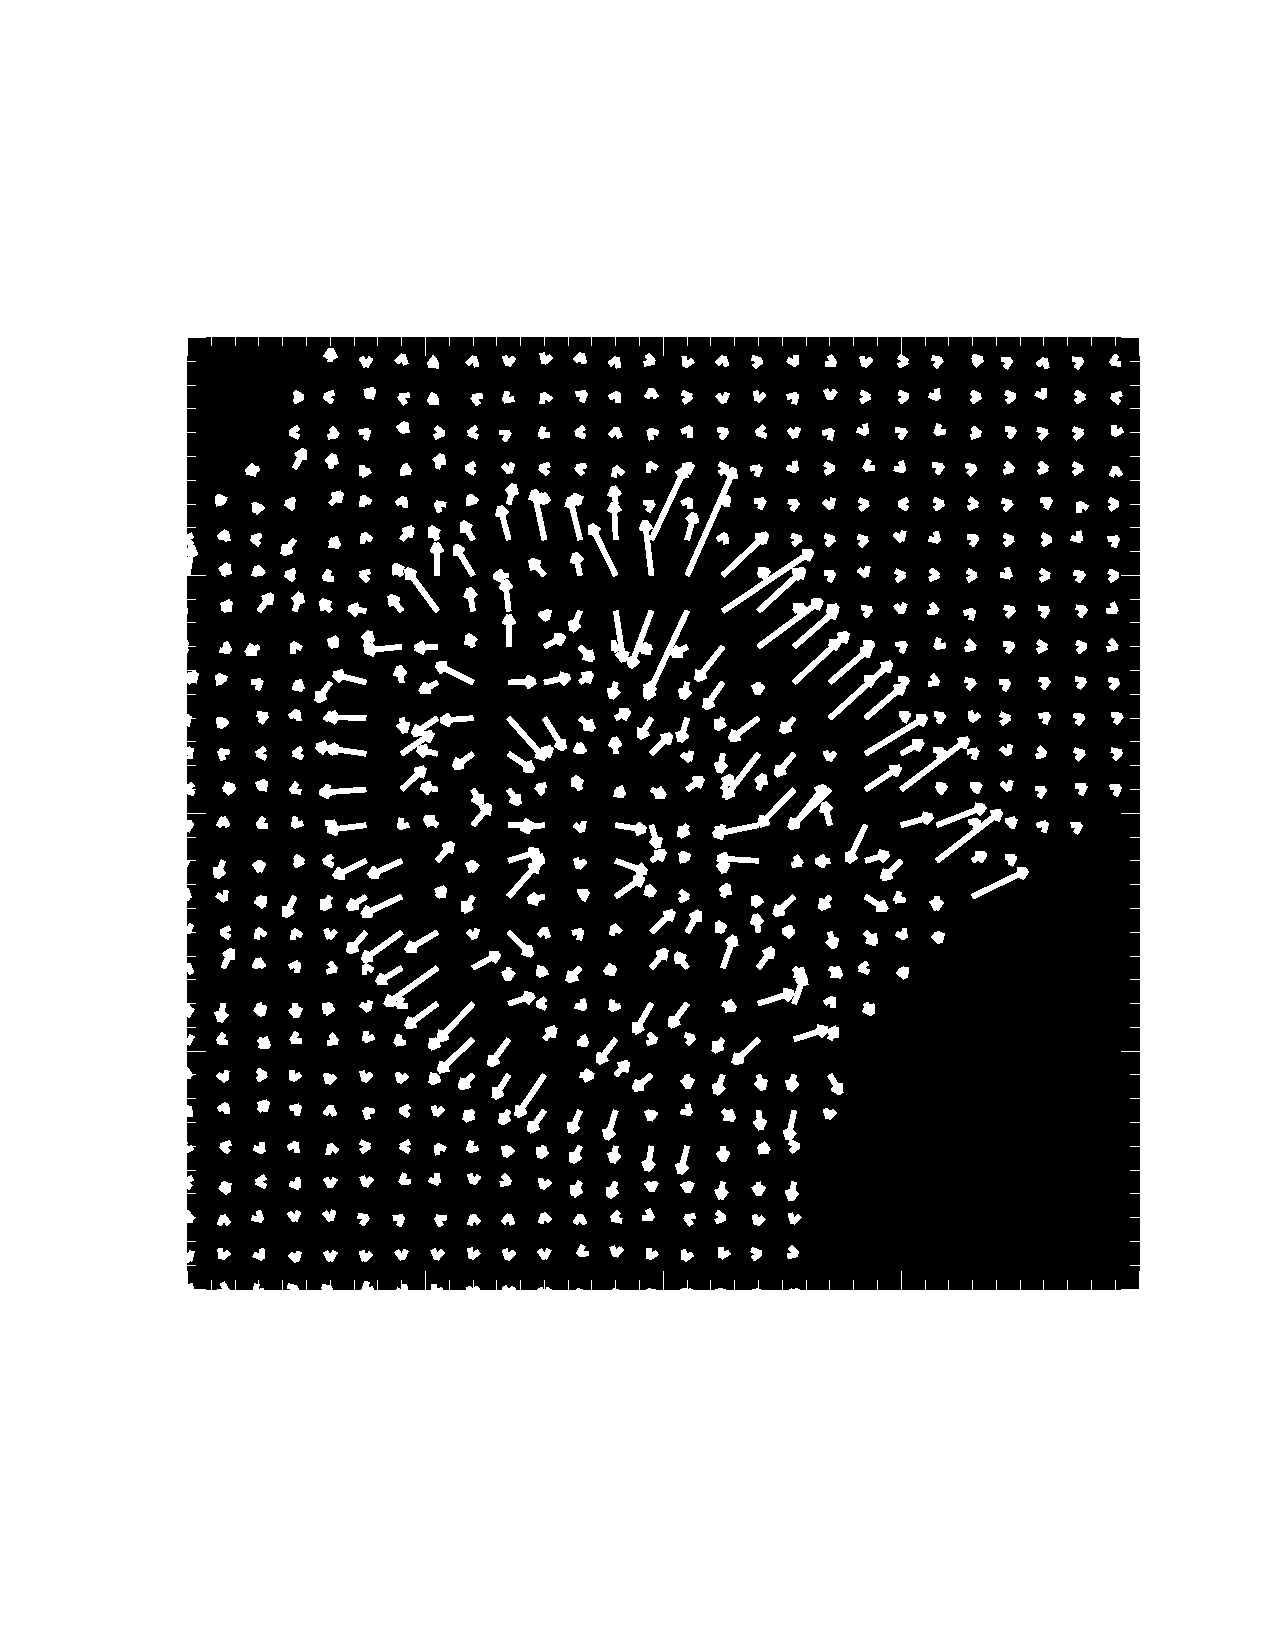
\includegraphics[scale=0.35, trim=55 130 80 130]{images/arrow2.pdf}
%}
%\caption{The vectors plotted represent the magnitude and angle determined from the gradient space of the high-pass filtering at a particular scale. The CME of 2004 April 1 shown here is highlighted very effectively by this method \citep{2009A&A...495..325B}.}
%\label{Vectors}
%\end{figure} 

At a particular scale the signal-to-noise ratio of the CME is highest and this is the optimum scale for determining the edges in the image. The angular component $\alpha$ of the gradient specifies a direction which points across the greatest intensity change in the data (an edge). A threshold is specified with regard to this gradient direction in order to chain pixels along maxima to highlight the edges. The changes in magnitude and angular information may then be implemented in a spatio-temporal filter for distinguishing those edges corresponding to the CME only. Overlaying a mesh of vector arrows on the data shows how the combined magnitude and angular information illustrate the progression of the CME. Each vector is rooted on a pixel in the gradient space, and has a length corresponding to the magnitude $M$ with an angle from the normal $\alpha$ (Figure~\ref{Vectors}). Using this information, it becomes possible to create a specific detection mask which is used to identify the edges along the CME front to study its propagation (as done for a sample of events in Chapter~\ref{chapter:kinematics}). However, for the cases of faint CMEs or strong streamer deflections, the filter is presently limited by exploiting the information from only one scale and ignoring all other scales, meaning it currently often requires the user to remove/include certain edges that the algorithm has mistakenly retained/discarded. Extending the algorithm to work on more than one scale may help alleviate this issue in order to develop a fully automated CME detection and characterisation routine, as outlined in the following section.

\subsection{Automated Multiscale CME Detection}
\label{automatedmultiscale}

For the most part, CMEs exist on size scales larger than noise and any small scale features in coronagraph images, such as stars or planets, that are redundant for studying CME propagation. This fact has led to the development and implementation of multiscale decompositions that highlight the CME in images from SOHO/LASCO and STEREO/SECCHI \citep{2008SoPh..248..457Y, 2009A&A...495..325B, 2003A&A...398.1185S}. However, coronal streamers (plasma outflows from open magnetic field regions on the Sun) can persist through coronagraph images with significant brightness intensities and tend to appear on similar scales as the CME in multiscale image analysis. If a CME propagates through an image with a strong streamer present, it becomes difficult to distinguish the two features by intensity thresholding alone, and this is one reason why differencing techniques have been widely used in CME analysis. In an effort to move away from differencing and the large errors involved in the subtraction of images from each other, since the goal is to obtain kinematics with the greatest precision, we endeavour to separate CME and streamer features from one another using multiscale methods alone. These efforts involve exploiting the angular distribution that exists across a curved CME front compared to the more linear streamers in single independent images. To do this, the coronagraph images must first be normalised for their radial gradient in intensity, since the drop-off across the field-of-view is too steep to effectively segment a single entire streamer from the inner to outer edge of an image. This can serve to enhance the noise at the edge of the images, but this is again suppressed by the multiscale analysis. Occasions when the CME propagates directly in front of, or behind, a streamer remain problematic, as do strong streamer deflections that can occur when a CME propagates into or expands alongside a streamer.

\subsection{Normalising Radial Graded Filter (NRGF)}

Since the brightness drop-off of the corona is large, falling from approximately $10^{-6}$\,--\,$10^{-9}$~B$_{\odot}$ across heights of 1\,--\,6~R$_{\odot}$ \citep{1998EP&S...50..493K}, a method for radially normalising coronagraph images to enhance features across this steep intensity gradient was developed by \citet{2006SoPh..236..263M}. It works by normalising the intensity in radial coordinates of the image according to the equation
\begin{eqnarray}
I'(r,\phi)\,=\,\frac{I(r,\phi)-I(r)_{<\phi>}}{\sigma(r)_{<\phi>}}
\end{eqnarray}
where $I'(r,\phi)$ is the processed and $I(r,\phi)$ is the original intensity at height $r$ and position angle $\phi$, and $I(r)_{<\phi>}$ and $\sigma(r)_{<\phi>}$ are the mean and standard deviation of intensities calculated over all position angles at height $r$. Figure~\ref{im+filt} shows the result when the NRGF is applied to a LASCO/C2 image of the 1 April 2004 CME.
\begin{figure}[!ht]
\resizebox{\hsize}{!}{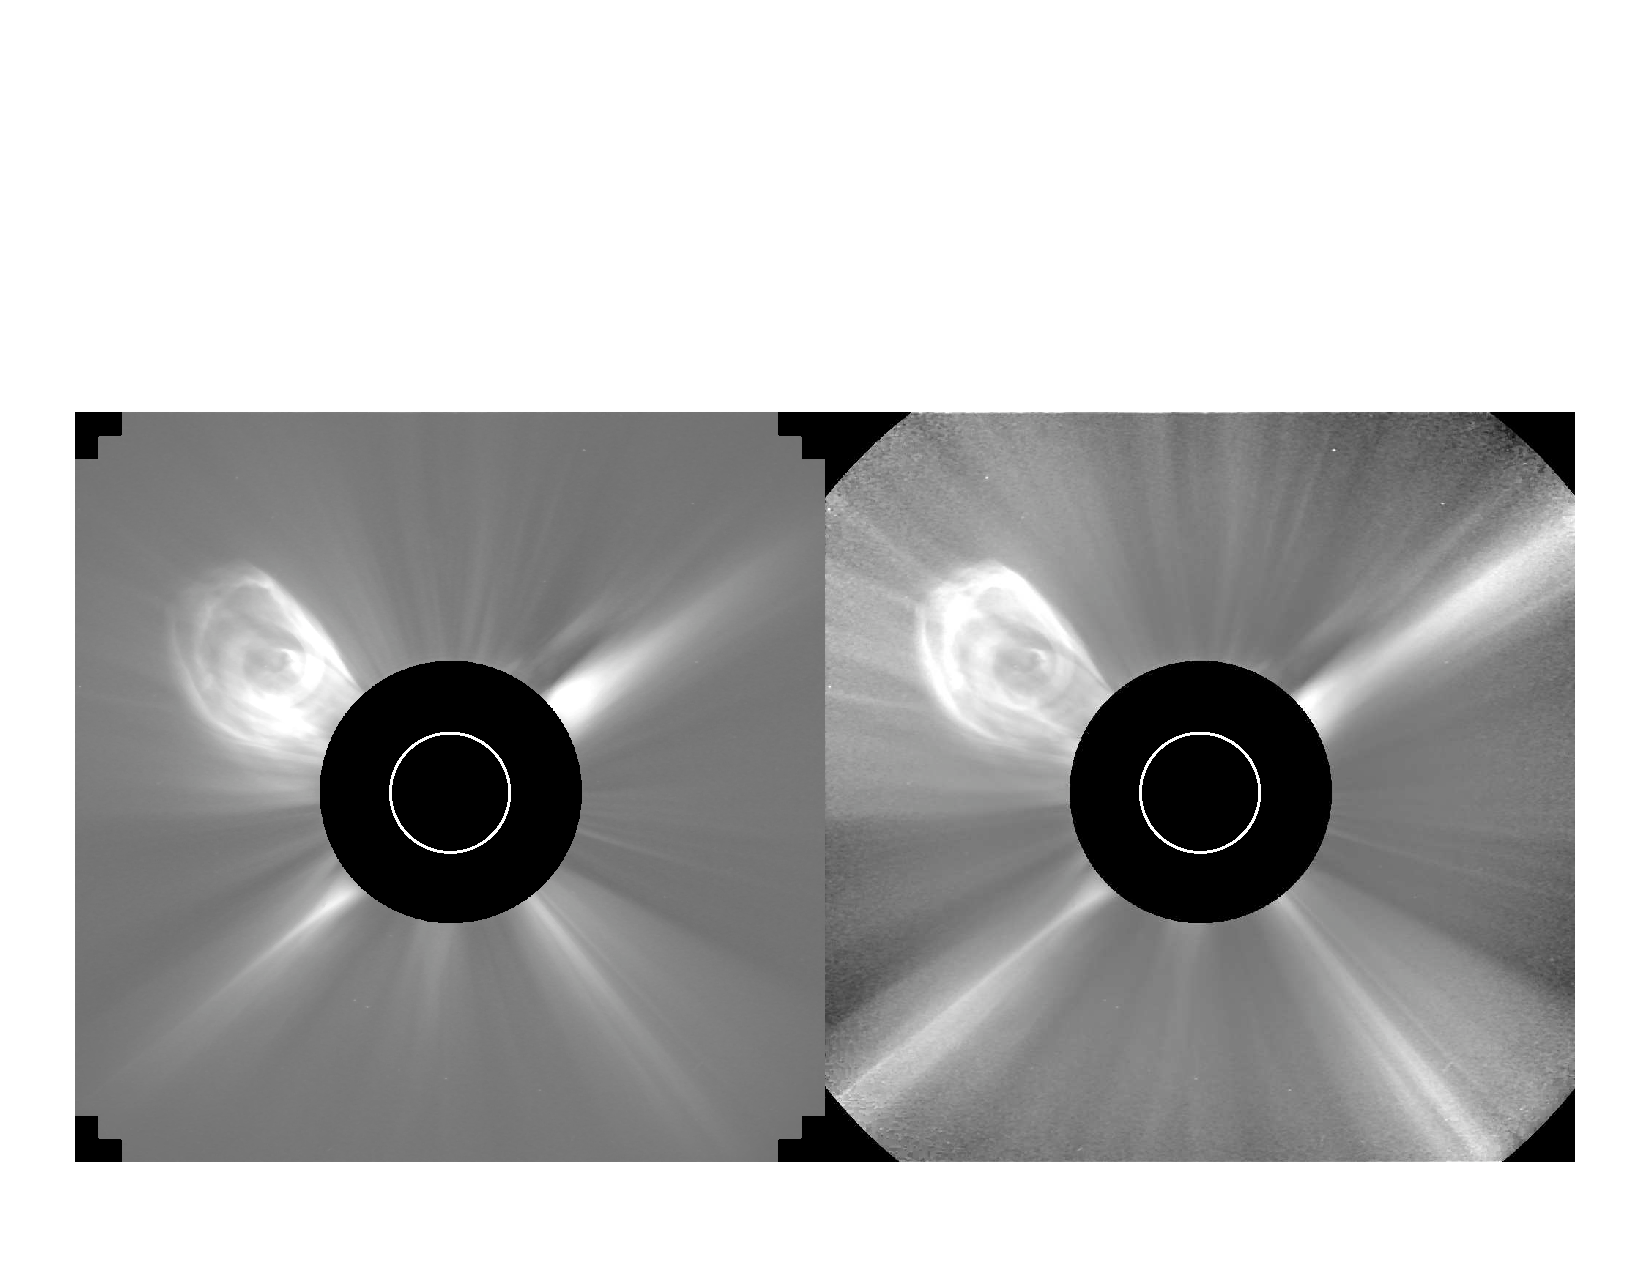
\includegraphics[clip=true, trim=30 50 30 190]{images/im+filt.pdf}}
\caption{A normalised, background subtracted, LASCO/C2 image (left) of a CME on 1 April 2004, and the resulting NRGF image (right). The image radial intensity is scaled such that structure along streamers and the CME becomes visible across the field-of-view}
\label{im+filt}
\end{figure}
\newline
\indent The multiscale decomposition introduced in \citet{2008SoPh..248..457Y} provides magnitude and angular information of the edges in the image. This information is combined to chain the strongest edges within the image on a scale that provides an optimal signal-to-noise ratio for studying the CME. \citet{2009A&A...495..325B} obtain the CME front edges in this manner, which are then used to fit an ellipse to characterise the CME propagation in the image sequence. In order to automate the algorithm, thresholds on the magnitude information (e.g., CME edges appear on larger scales than noisy features) and angular information (e.g., CME edges appear more curved than streamer edges) were investigated. The thresholding is strengthened by the inclusion of more than one scale in localising the CME and distinguishing it from the streamers, detailed below.

\subsubsection{Thresholding}

\begin{figure}[!ht]
\resizebox{\hsize}{!}{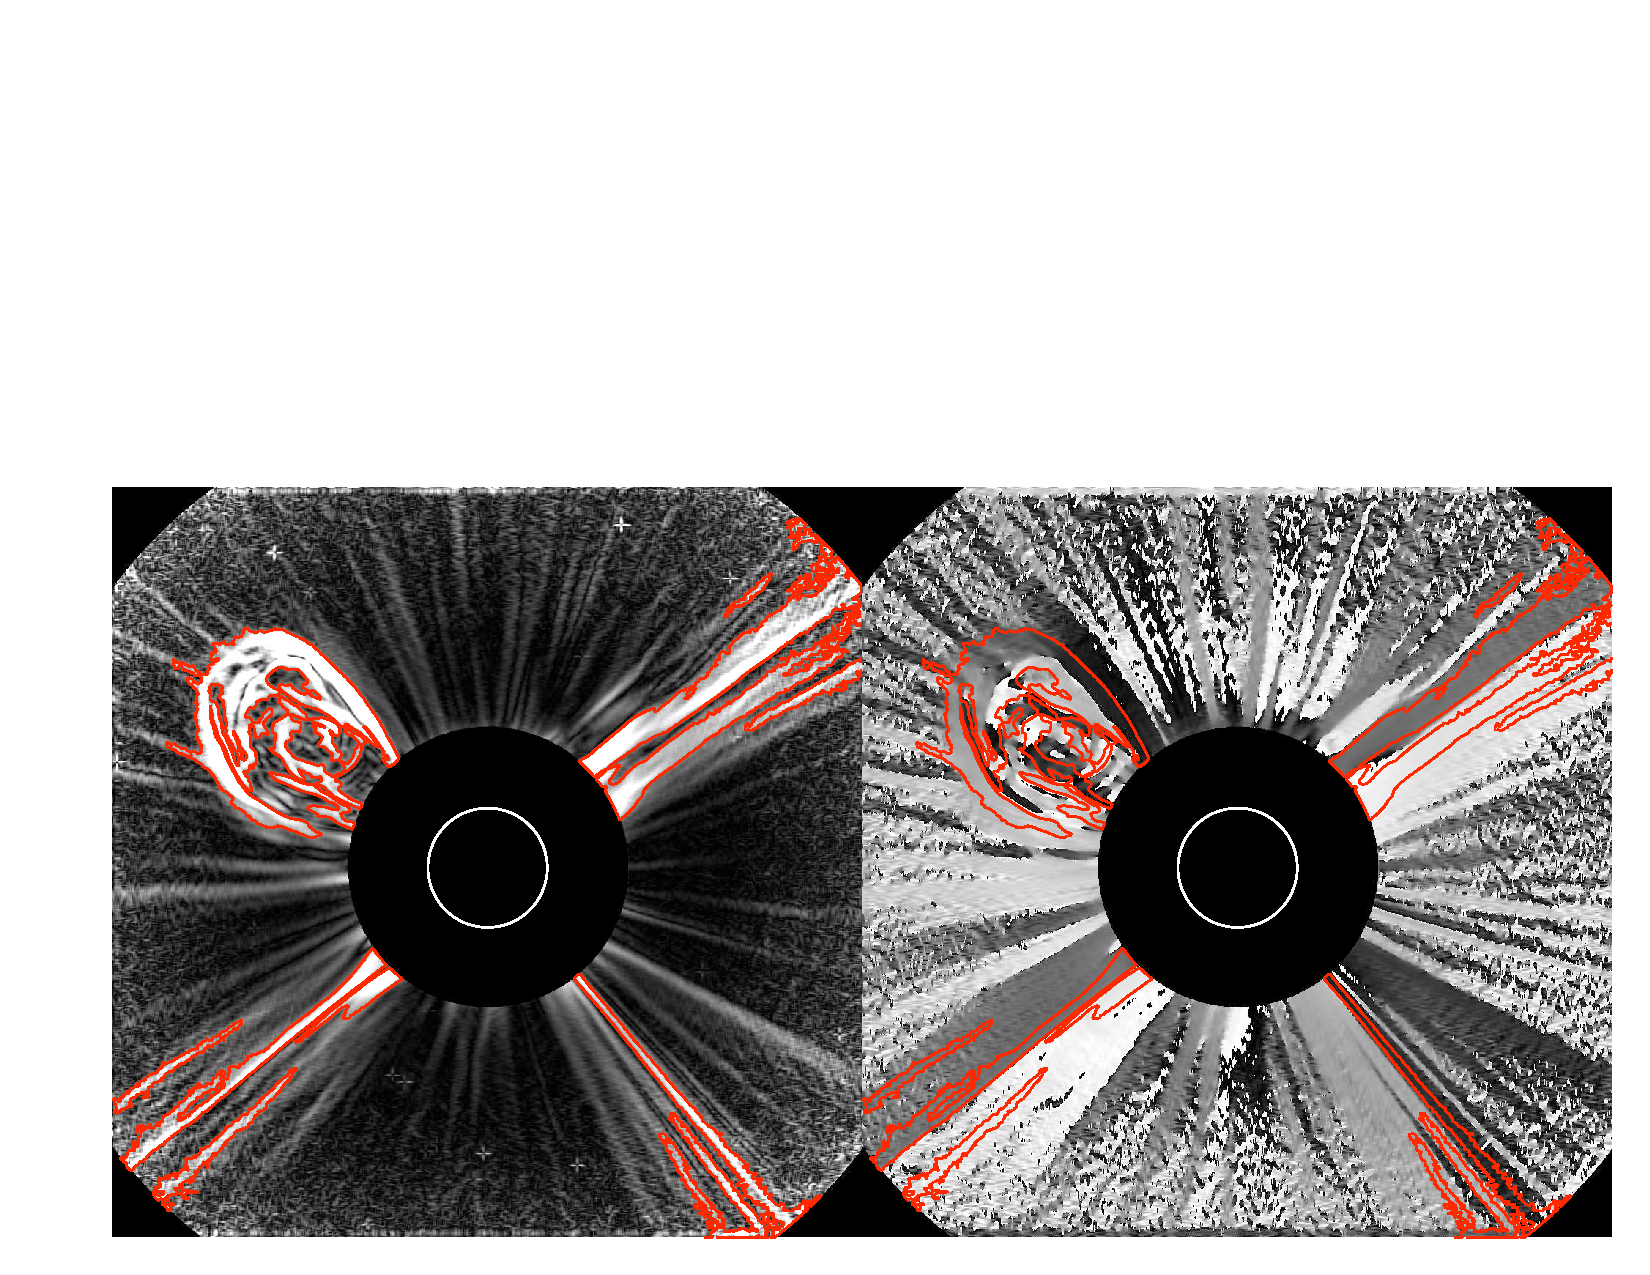
\includegraphics[clip=true, trim=40 20 0 230]{images/modalpmapcontour.pdf}}
\caption{A chosen scale of the decomposed NRGF image provides a magnitude image of the edge strengths displayed on the left, which is thresholded at one standard deviation from the mean intensity to obtain contoured regions of interest that could contain a CME (sample contours indicated in red). As shown, the streamers have edges which appear on the same scale as the CME edges in this image. The angular information from the decomposition is displayed on the right, and the contoured regions of interest overlaid for comparison. The grey scale indicates angles from 0\,--\,360$^{\circ}$ and it is clear that streamers tend to have a linear grey scale while the CME has a gradient of greys across the scale.}
\label{modalpmapcontour}
\end{figure}

The magnitude information corresponds to the strength of the edges in the image, and so can be thresholded to discard the small scale noise. For the NRGF image (Figure~\ref{im+filt}), a hard threshold $T$ is set at one standard deviation $\sigma$ of the mean $\mu$ of the image intensity to contour regions of interest that may be a CME according to the equations:
\begin{equation}
T \,=\, \mu + N \sigma \,=\, \underbrace{ \frac{1}{n}\sum_{i=1}^n x_i}_{\mbox{mean}} \,+ N \underbrace{ \sqrt{ \frac{1}{n} \sum_{i=1}^n \left( x_i - \mu \right) ^2 } }_{\mbox{standard deviation}}
\label{eqn:threshold}
\end{equation}
where $x_i$ are the pixel intensity values of the image, and we choose the number of standard deviations $N=1$. The left image of Figure~\ref{modalpmapcontour} illustrates this thresholding with a sample of contoured regions (outlined in red) on the multiscale decomposition of a CME observed in LASCO/C2 on 1 April 2004.
\begin{figure}[!t]
\centerline{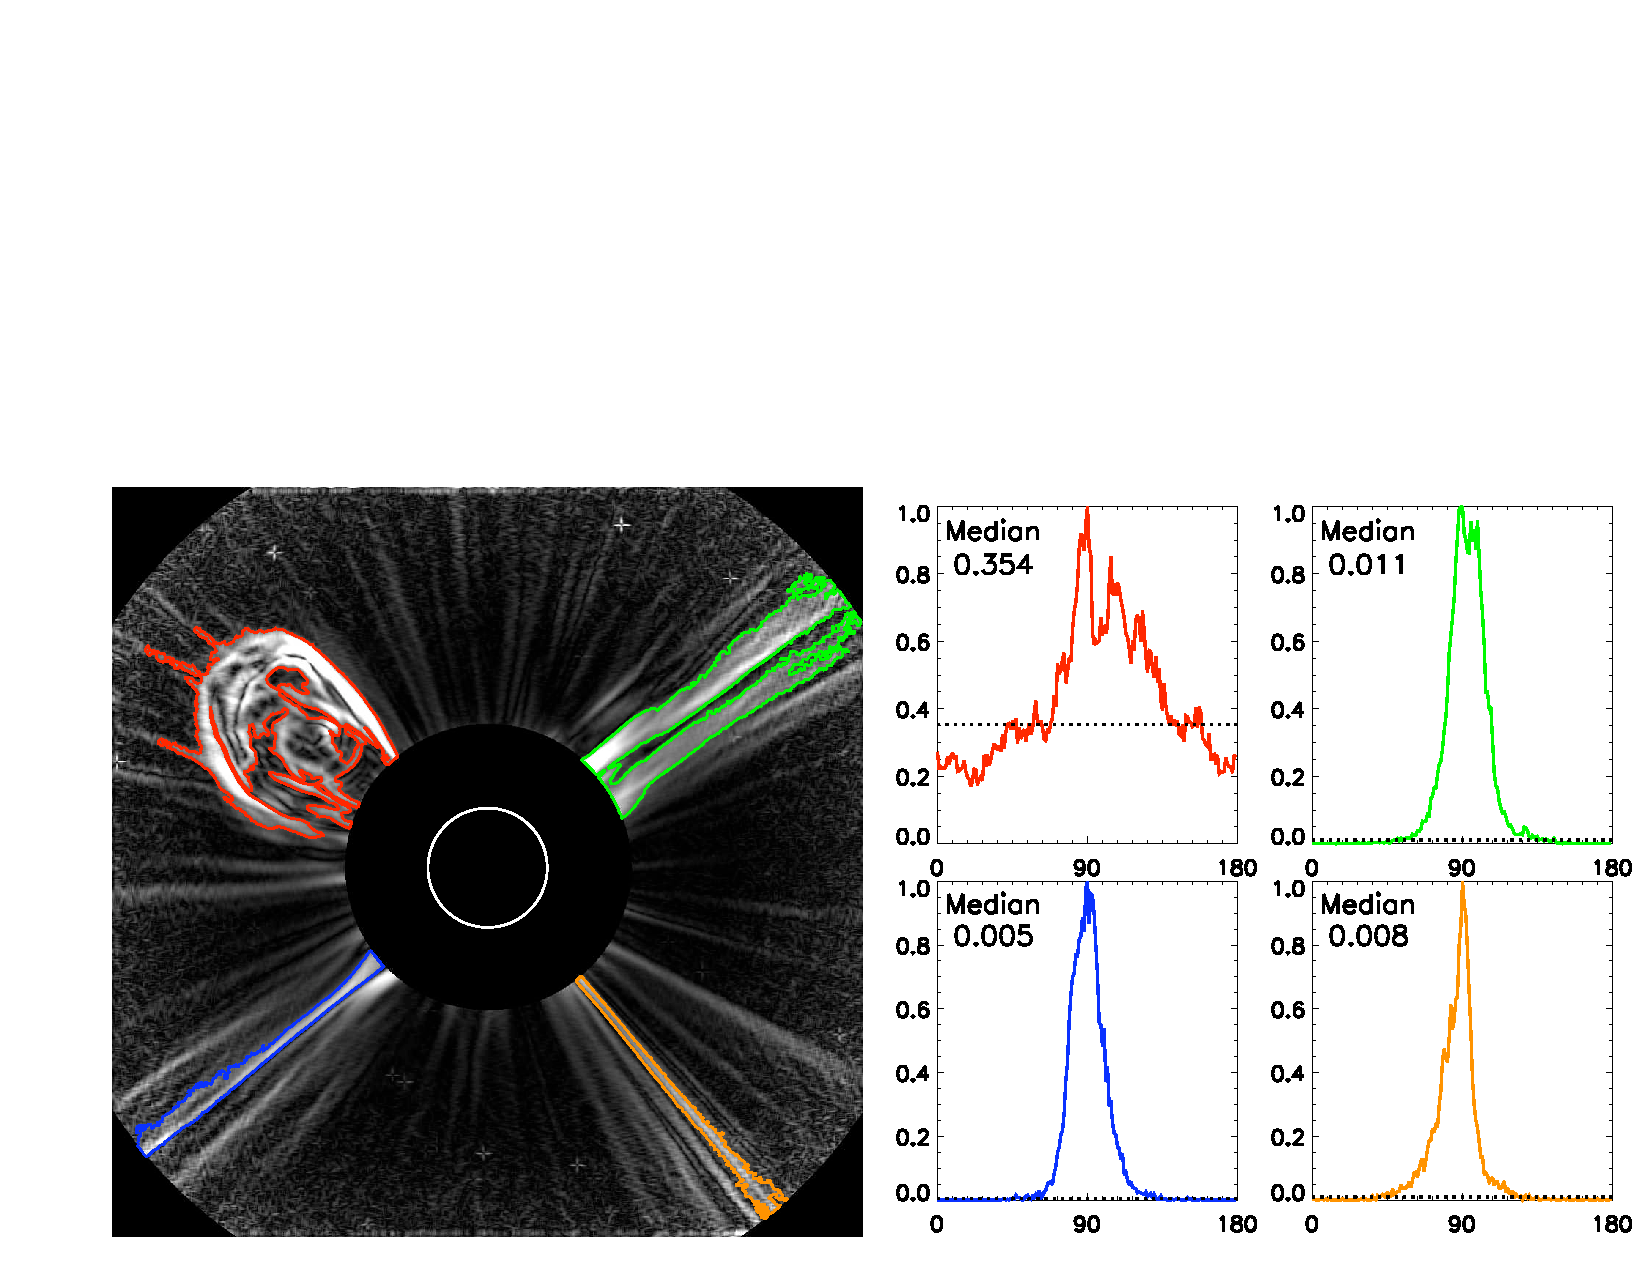
\includegraphics[scale=0.55, clip=true, trim=40 20 0 230]{images/colour_contours_distributions.pdf}}
\caption{Left: four contoured regions (at one standard deviation of the mean image intensity) highlighted on the magnitude information from the multiscale decomposition of the 1 April 2004 CME. Right: the corresponding angular distribution of each region, normalised and folded into the 0\,--\,180$^{\circ}$ range (centred on 90$^{\circ}$). The angular distribution may be thresholded with respect to its median value to distinguish regions corresponding to CMEs from those along streamers.}
\label{ccdistributions}
\end{figure}

It is apparent from the right of Figure~\ref{modalpmapcontour} that the CME will contain edges whose normals are widely distributed across 0\,--\,360$^{\circ}$ compared to the more linear, radially directed, streamer edges. The angular distribution of each region is determined and then normalised and folded into 0\,--\,180$^{\circ}$ range, centred on 90$^{\circ}$, due to the symmetry of the edge normals. This is illustrated for four selected contour regions in Figure~\ref{ccdistributions}. The resulting angular distributions are then thresholded with regard to their median value, since the distribution of angles across the CME will be wider and have a higher median value than for a distribution of angles along a streamer.

This thresholding is repeated across four scales of the multiscale decomposition, neglecting smaller scales dominated by noise and larger scales that are overly smoothed. Assigning a score to the regions that may contain a CME at each scale, it becomes possible to build a detection mask as in Figure~\ref{cme_mask}. 
\begin{figure}[!t]
\centerline{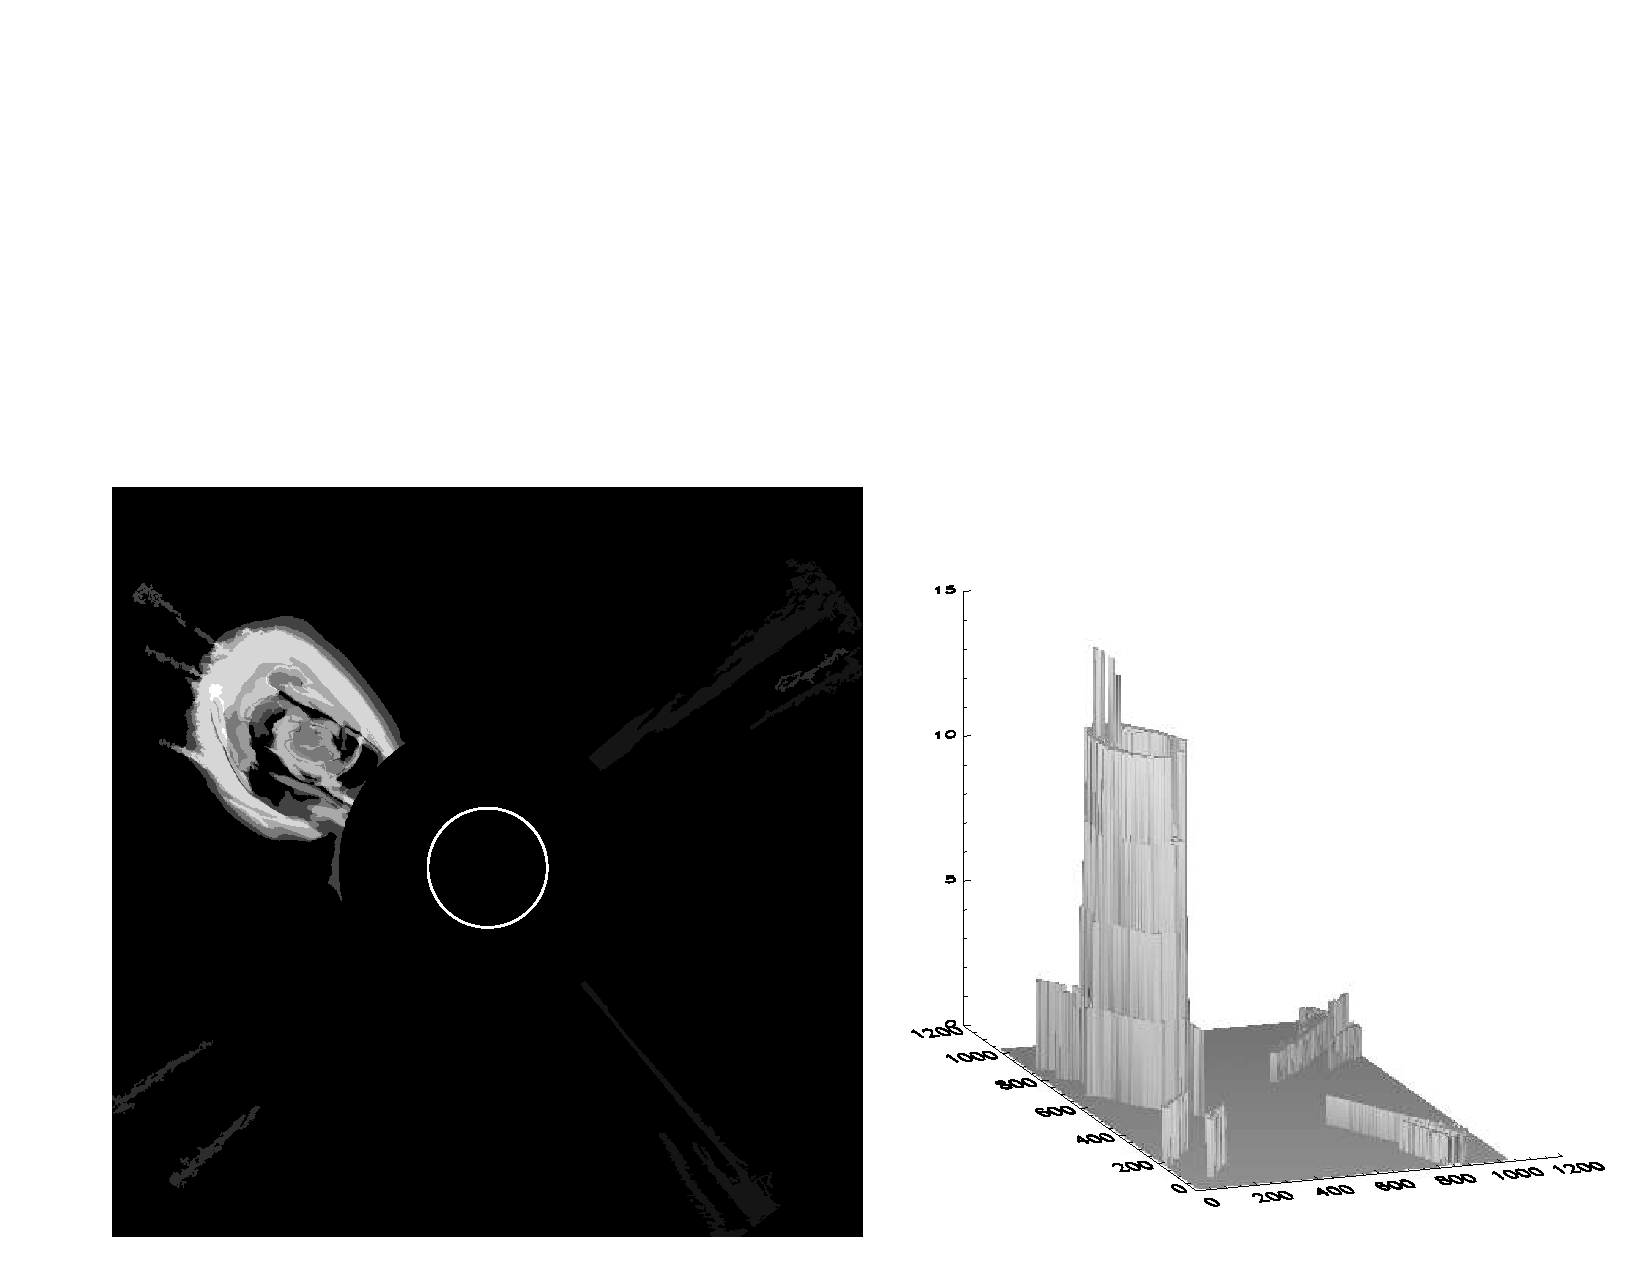
\includegraphics[scale=0.55, clip=true, trim=40 20 0 230]{images/cme_mask.pdf}}
\caption{The resulting CME detection mask from combining the thresholded regions of strongest magnitude and angular distribution at four scales of the decomposition. The 3D representation on the right illustrates the pixel values of the mask.}
\label{cme_mask}
\end{figure}

The scoring system is chosen arbitrarily to work best with the chosen thresholds, and these may be changed and refined as an analysis of more CMEs is done. For example, the current thresholds from working on a sample of $\sim$\,10 CMEs are as follows:
\begin{enumerate}
\item The magnitude information is thresholded at one standard deviation (1$\sigma$) of the mean intensity across the image.
\item The 15 largest contoured regions across the image are investigated (there are rarely more than $\sim$\,5 streamers of similar intensity to a CME, and we allow for disjointed contours along structures). 
\item If the median angular value is $>$\,20\% of the angular distribution peak then the region is deemed a CME and assigned a score of 3 (the pixels in that region of the mask are given the value 3). 
If it is $>$\,10\% the score is 2 (potential CME structure), or $>$\,5\% the score is 1 (weak CME structure or portion thereof).
\item The final CME mask through the combination of scores at each scale results in a dominant region that localises the CME front in the image and can be used to characterise the front, or input into a spatio-temporal filter if subsequent CME images are available in order to refine the masked region whenever streamers are still present. 
\end{enumerate}
The resultant set of detection masks for three of the frames of the CME observed on 1 April 2004 are shown in Figure~\ref{20040401_cme_masks}.

\begin{figure}[p]
\centerline{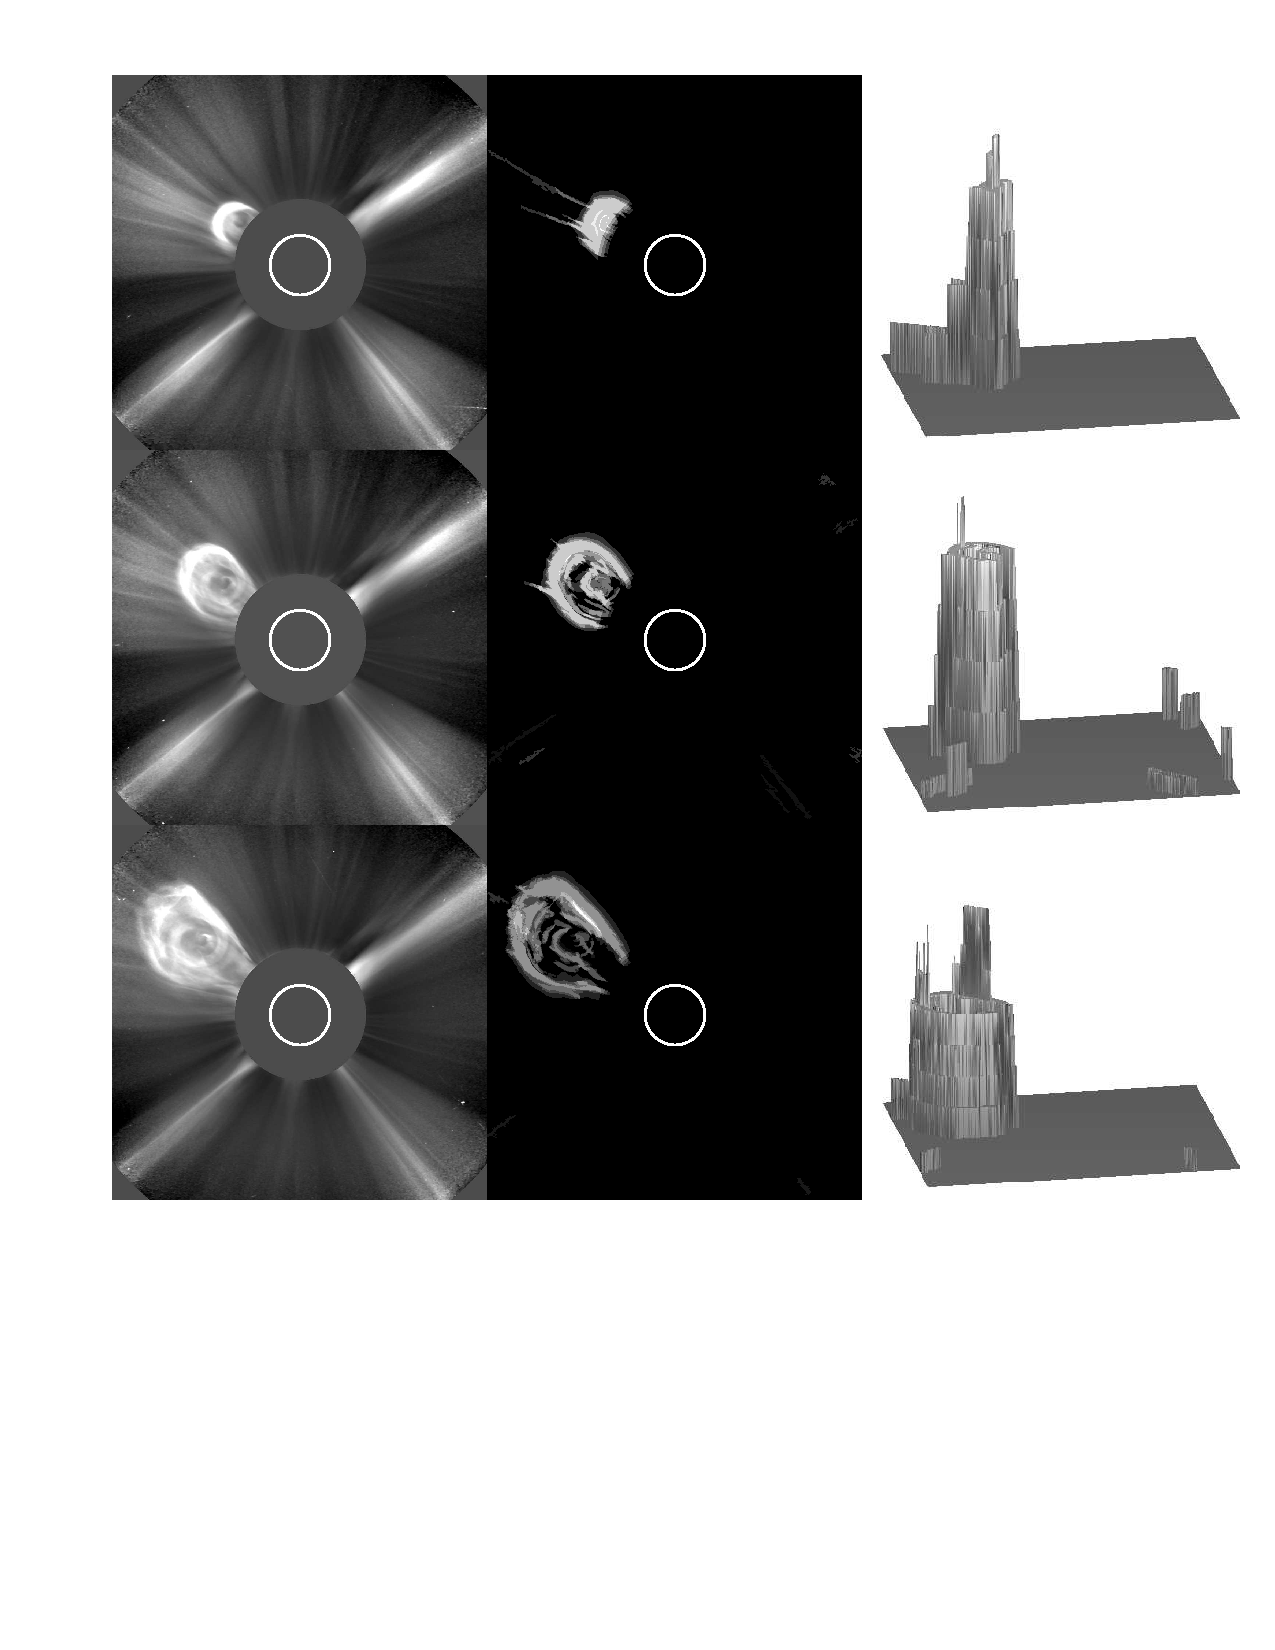
\includegraphics[scale=0.75, clip=true, trim=40 200 0 0]{images/20040401_cme_masks.pdf}}
\caption{The NRGF (left) and resulting detection masks (middle and right) for different frames of a CME observed by LASCO/C2 at times of 00:00~UT (top), 00:40~UT (middle) and 01:20~UT (bottom) on 2 April 2004. The location of the CME front is highlighted very efficiently by this method, although the detection masks may contain artefacts of the chosen thresholds which must be discarded when characterising the CME front.}
\label{20040401_cme_masks}
\end{figure}

\subsubsection{Faint CMEs and Streamer Interactions/Deflections}

\begin{figure}[!p]
\centerline{\includegraphics[scale=0.82, clip=true, trim=0 90 90 55]{images/20010423_faint.pdf}}
\caption{Example of the difficulty in detecting the faint CME observed by LASCO on 23 April 2001. If the CME is far-sided and/or of low intensity it becomes difficult to threshold its edges in the image compared to the coronal streamers. ({\bf a}) is the pre-processed CME image. ({\bf b}) is the NRGF image. ({\bf c}) and ({\bf d}) show the magnitude and angular information from the multiscale decomposition with intensity contours overlaid in red. ({\bf e}) and ({\bf f}) show the resulting CME detection mask in 2D and 3D respectively.}
\label{faintCME}
\end{figure}

Due to the nature of the hard thresholds in place on the magnitude and angular information, there are problems which arise when the algorithm mistakenly disregards a CME or includes a streamer, or portions thereof. Firstly, if a CME is faint enough that the intensity falls below the 1$\sigma$ magnitude threshold, it will not be detected as a region of interest in the image. Secondly, if the CME interacts with a streamer, the two features may be contoured together and this will skew the angular distribution and affect the detection mask. And thirdly, if the CME causes a significant streamer deflection, it will lead to a wider distribution of angles along the streamer and the algorithm may thus detect it as part of the CME. This is why the above scoring system was introduced in an effort to minimise these effects, which are highlighted in Figure~\ref{faintCME} for a CME observed on 23 April 2001. The event is too faint compared with the streamers across it for it to be easily distinguished in the image, and parts of the streamers are then mistakenly included in the final detection mask. This is where the current algorithm requires a user to specify which parts of the edges correspond to the CME for characterisation. Such limitations in current wavelet analysis of CMEs may be overcome by extending these algorithms to work with ridgelets or curvelets that better suit the curved form of a typical CME front as discussed in \citet{2010gallagher}. Furthermore, it should be noted that a relatively small number of CMEs exhibit a narrow, spiky or strongly kinked structure which may not be readily distinguished from streamers in an automated fashion, nor have an adequately high angular distribution for automatic detection in the images. These CMEs may also not be satisfactorily characterised with an ellipse, discussed in the following section, however they are not typical of the commonly observed curved nature of CMEs and thus represent a small class of events outside the limits of these methods as they currently stand.



%% Figure 
%
% \begin{figure} 
% \centerline{\includegraphics[width=0.5\textwidth,clip=]{<fig.eps>}}
% \caption{}%\label{fig:?}
% \end{figure}



%% Table
%
% \begin{table}
% \caption{}%\label{tbl:?}
% \begin{tabular}{}     
% \hline
% \multicolumn{2}{c}{<>}
% <data>
% \hline
% \end{tabular}
% \end{table}
  

%%%%%%%%%%%%%%%%%%%%%%%%%%%%%%%%%%%%%%%%%%%%%%%%%%%%%%%%%%%%%%%%%%%%%%%%%%%
%% Appendix
%
% \appendix   



%%%%%%%%%%%%%%%%%%%%%%%%%%%%%%%%%%%%%%%%%%%%%%%%%%%%%%%%%%%%%%%%%%%%%%%%%%%
%% Acknowledgements
%
% \begin{acks}
%
% \end{acks}


%%% %%%%%%%%%%%%%%%%%%%%%%%%%%%%%%%%%%%%%%%%%%%%%%%%%%%%%%%%%%%
%% Bibliography
%
% Using BibTeX
%
 \bibliographystyle{spr-mp-sola.bst}
% %\bibliographystyle{spr-mp-sola-cnd} %% Alternative style: no title, no concluding page
 \bibliography{references.bib}  
%
% Without BibTeX 
% \begin{thebibliography}{}
% \bibitem[\protect\citeauthoryear{Author}{Year}]{key}
%   <bibliographical entry>
%
% \bibitem[\protect\citeauthoryear{}{}]{}
%   
%  
% \end{thebibliography}

\end{article} 
\end{document}
